% UTF-8 encoding
% Compile with latex+dvipdfmx, pdflatex, xelatex or lualatex
% pdflatex is recommanded
% This template is released under BSD 2-Clause license.
\documentclass[UTF8]{ctexart}
\usepackage{xcolor}

% 自定义的一些颜色
\definecolor{hyperref-green}{RGB}{0,150,0}
\definecolor{hyperref-red}{RGB}{200,0,0}

% 超链接
\usepackage[pagebackref=true,breaklinks=true,citecolor=hyperref-green,linkcolor=hyperref-red,menucolor=black,letterpaper=true,colorlinks,bookmarks=false]{hyperref} 
\usepackage{bibentry}

\usepackage{pdfpages} % includepdf

%% 公式和数学标识相关%%%%%%%%%%%%%%%%%%%%%%%%%%%%%%%%%%%%%%%%%%%%%%%%%
\usepackage{amsmath}
\usepackage{xcolor} % math color
\numberwithin{equation}{section} % 公式按章节编号
\numberwithin{table}{section} % 公式按章节编号

% 声明argmin运算符
\DeclareMathOperator*{\argminA}{arg\,min} % Jan Hlavacek
\DeclareMathOperator*{\argminB}{argmin}   % Jan Hlavacek
\DeclareMathOperator*{\argminC}{\arg\min}   % rbp
\usepackage{amsfonts}
%%%%%%%%%%%%%%%%%%%%%%%%%%%%%%%%%%%%%%%%%%%%%%%%%%%%%%%%%%%%%%%%%%

% 插入图表和图表描述
\usepackage{graphicx, caption, subfigure, float}
\DeclareCaptionFormat{myformat}{\fontsize{8}{8}\selectfont#1#2#3}
\captionsetup{format=myformat}
\captionsetup{margin=2cm}
\captionsetup{justification=centering}

% 将章节标号转为中文
\usepackage{zhnumber}  
%% geometry
\usepackage{geometry}
\geometry{left=3.17cm,right=3.17cm,top=3.0cm,bottom=3.0cm}  % 页边距

% 页眉相关的设置
\usepackage{fancyhdr}
\fancyhf{}  % 清除默认页眉
\pagestyle{fancy}
\lhead{上海大学硕士学位论文}  % 添加右侧页眉
\rhead{KAI ZHAO: \url{http://kaiz.xyz}}  % 右侧页眉,写你自己的论文的时候请去掉本行。
\cfoot{\thepage}  % 添加页脚页码

%% 设置章节格式
\CTEXsetup[name={第, 章}]{section}
\CTEXsetup[number={\chinese{section}}]{section}
\CTEXsetup[format+={\zihao{-2}}]{section}   % 大章节字体: 小二
\CTEXsetup[format+={\zihao{3}}]{subsection} % 小章节字体: 三号
\CTEXsetup[format+={\zihao{-4}}]{subsubsection}

% 绘制算法流程图
\usepackage{algorithm, algorithmic}

% 图表按章节编号
\usepackage{chngcntr}
\counterwithin{figure}{section}

\begin{document}
\zihao{-4} %
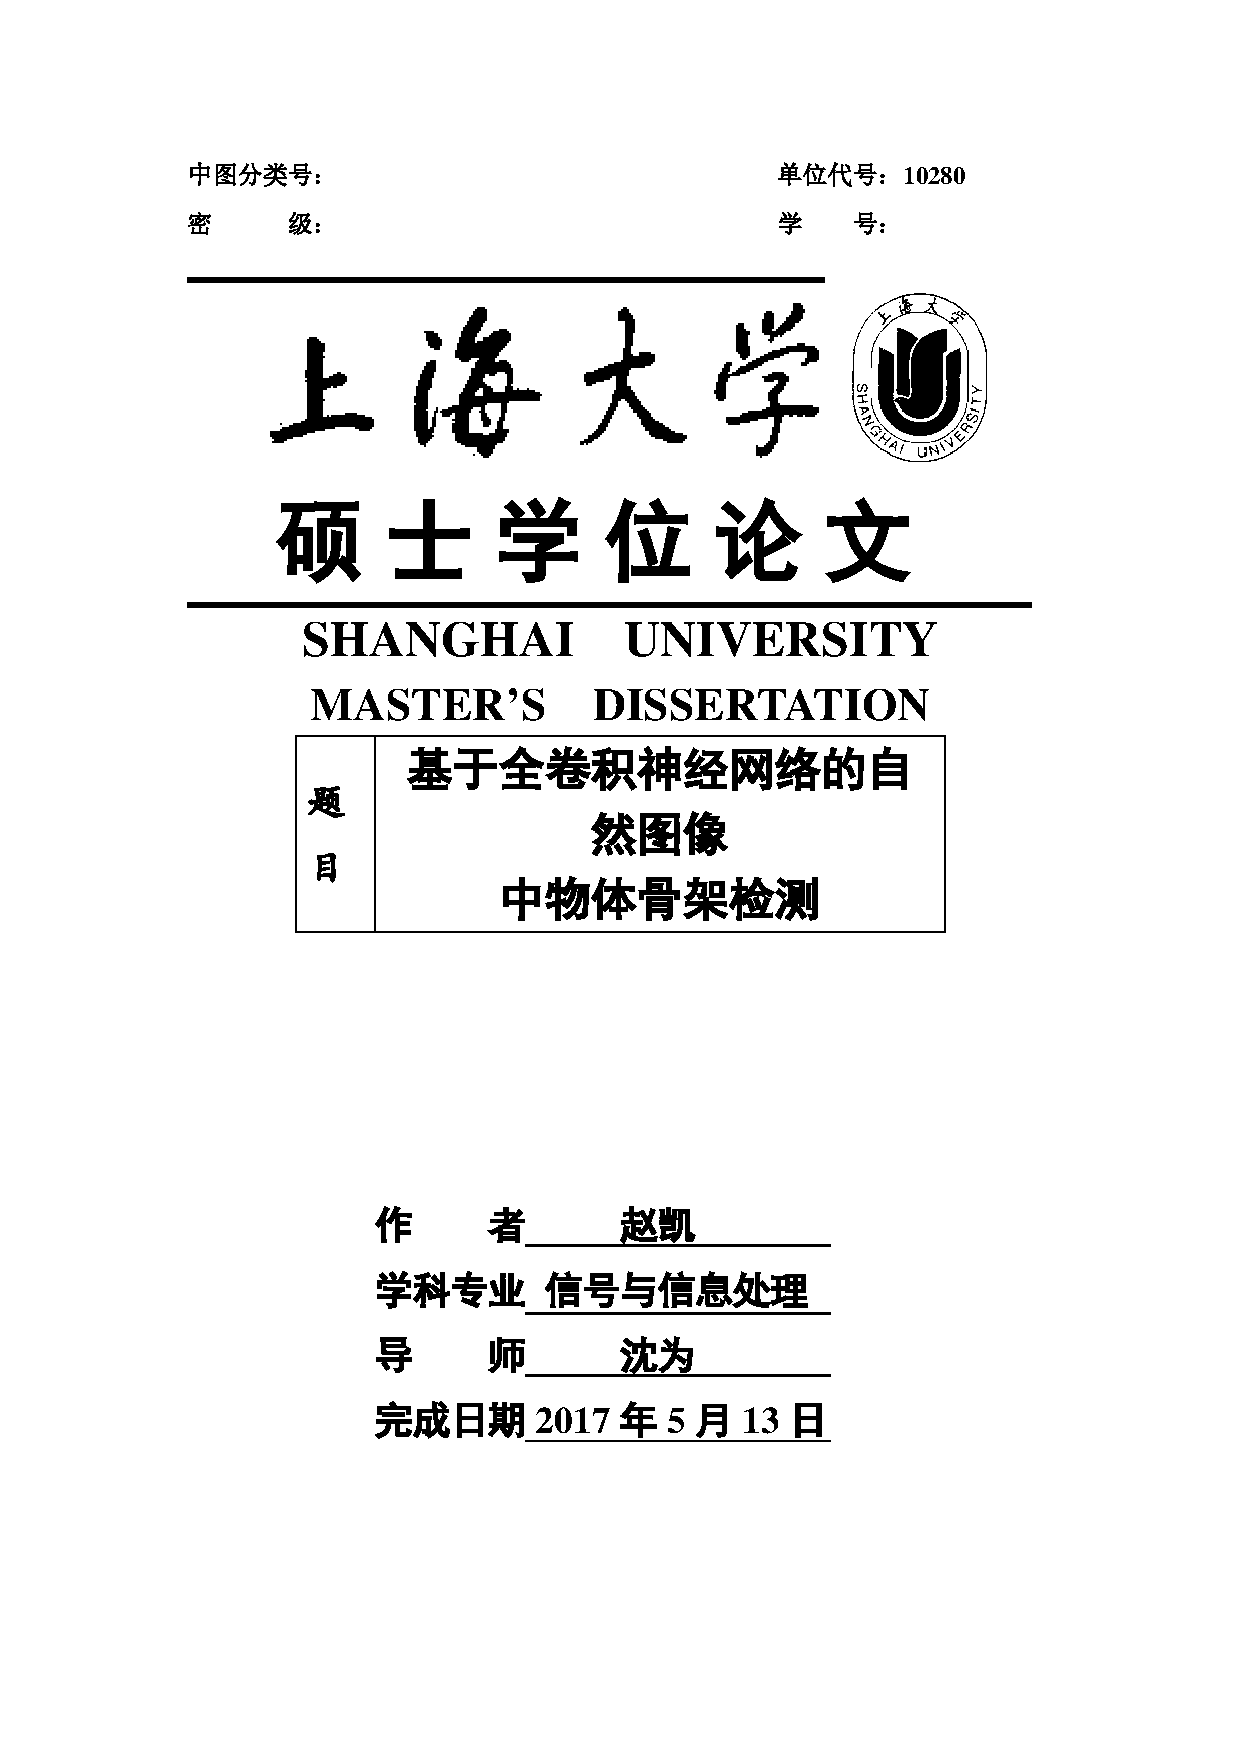
\includepdf[pages={1-9}]{cover.pdf}
\pagenumbering{Roman} % 导入封面内容
\setcounter{page}{9}  % LaTex的起始页码
%%%%%%%%%%%%%%%%%%%%%%%%%%%%%%%%%%%%%%%%%%%%%%%%%%%%%%%%%%%%%
% 此处请大家务必注意!!
% 由于本人能力/精力有限,并没有设计毕业论文‘目录之前的所有内容’
% 包括‘封面,中/英文摘要,原创说明,授权说明’等内容,
% 这些版面的设计也并非LaTex的长处。
% 因此这部分需要你使用学校的Word模板编写,然后导出pdf。
% 最后在latex中·includepdf[1-9]{your-awesome-cover.pdf}·
% 注意,上面的页码请根据你得到的pdf的实际页码填写。
% 还需注意,为了让word的页码和LaTex的页码连续(LaTex页码默认从1开始)
% 需要为LaTex手动设置起始页码
%%%%%%%%%%%%%%%%%%%%%%%%%%%%%%%%%%%%%%%%%%%%%%%%%%%%%%%%%%%%%

% 由于目录(TOC: table of contents)也会被hyperref作为超链接,因此颜色会被设置为和图表超链接一样的红色,红色的目录不好看。
% 这里单独把TOC的颜色设置为黑色。
{\hypersetup{linkcolor=black}
\tableofcontents}

%%%%%%%%%%%%%%%%%%%%%%%%%%%%%%%%%%%%%%%%%%%%%%%%%%%%%%%%%%%%%%%%%%%%%%%%%%%%%%%%%%%
%%%%%%%%%%%%%%%%%%%%%%%%%%%%%%%%%%%%%%%%%%%%%%%%%%%%%%%%%%%%%%%%%%%%%%%%%%%%%%%%%%%
\pagebreak
\section{绪论}
\pagenumbering{arabic} % 正文开始,页码使用阿拉伯数字
\setcounter{page}{1}
\subsection{课题研究的目的和意义}
计算机视觉研究的目的就是让计算机能像人类一样理解图像中的语义,\textbf{表示}和\textbf{识别}一直是计算机视觉研究中的两大热点。图像中往往包含大量信息,其中一部分对识别而言是关键信息,但是其中很大部分都是对识别无用的冗余信息。
所谓表示,就是人工提炼出其中的关键信息并且量化为计算机可以处理的数值形式。识别就是让计算机处理这些提炼出的有用信息并得到我们想要的语义,例如“判断图像某个位置是否存在人脸”,“判断照片拍摄的场景”等等。在模式识别和机器学习技
术引入到计算机视觉中后,经典的识别系统往往包含以下两个过程:(1)特征提取,(2)分类器训练。这其中“特征提取”就是一个\textbf{表示}的过程,而训练分类器的目的就是让计算机学会处理所提取的特征并识别其中的语义。针对不同的场景,科学
家们设计了大量的特征提取算法,例如用于图像物体轮廓检测的梯度和纹理特征~\cite{Lim_2013_CVPR}、用于人脸表示的LBP特征~\cite{ahonen2006face}等等。骨架作为一种高层次(high level)的特征,是物体形状和结构的简洁表示。由于骨架同时
包含物体的结构信息和物体部件之间的连接信息,而且骨架对非刚性形变具有不变性,因此在基于骨架的物体识别和表示中具有独一无二的优势。


\begin{figure}[!htb]
\centering
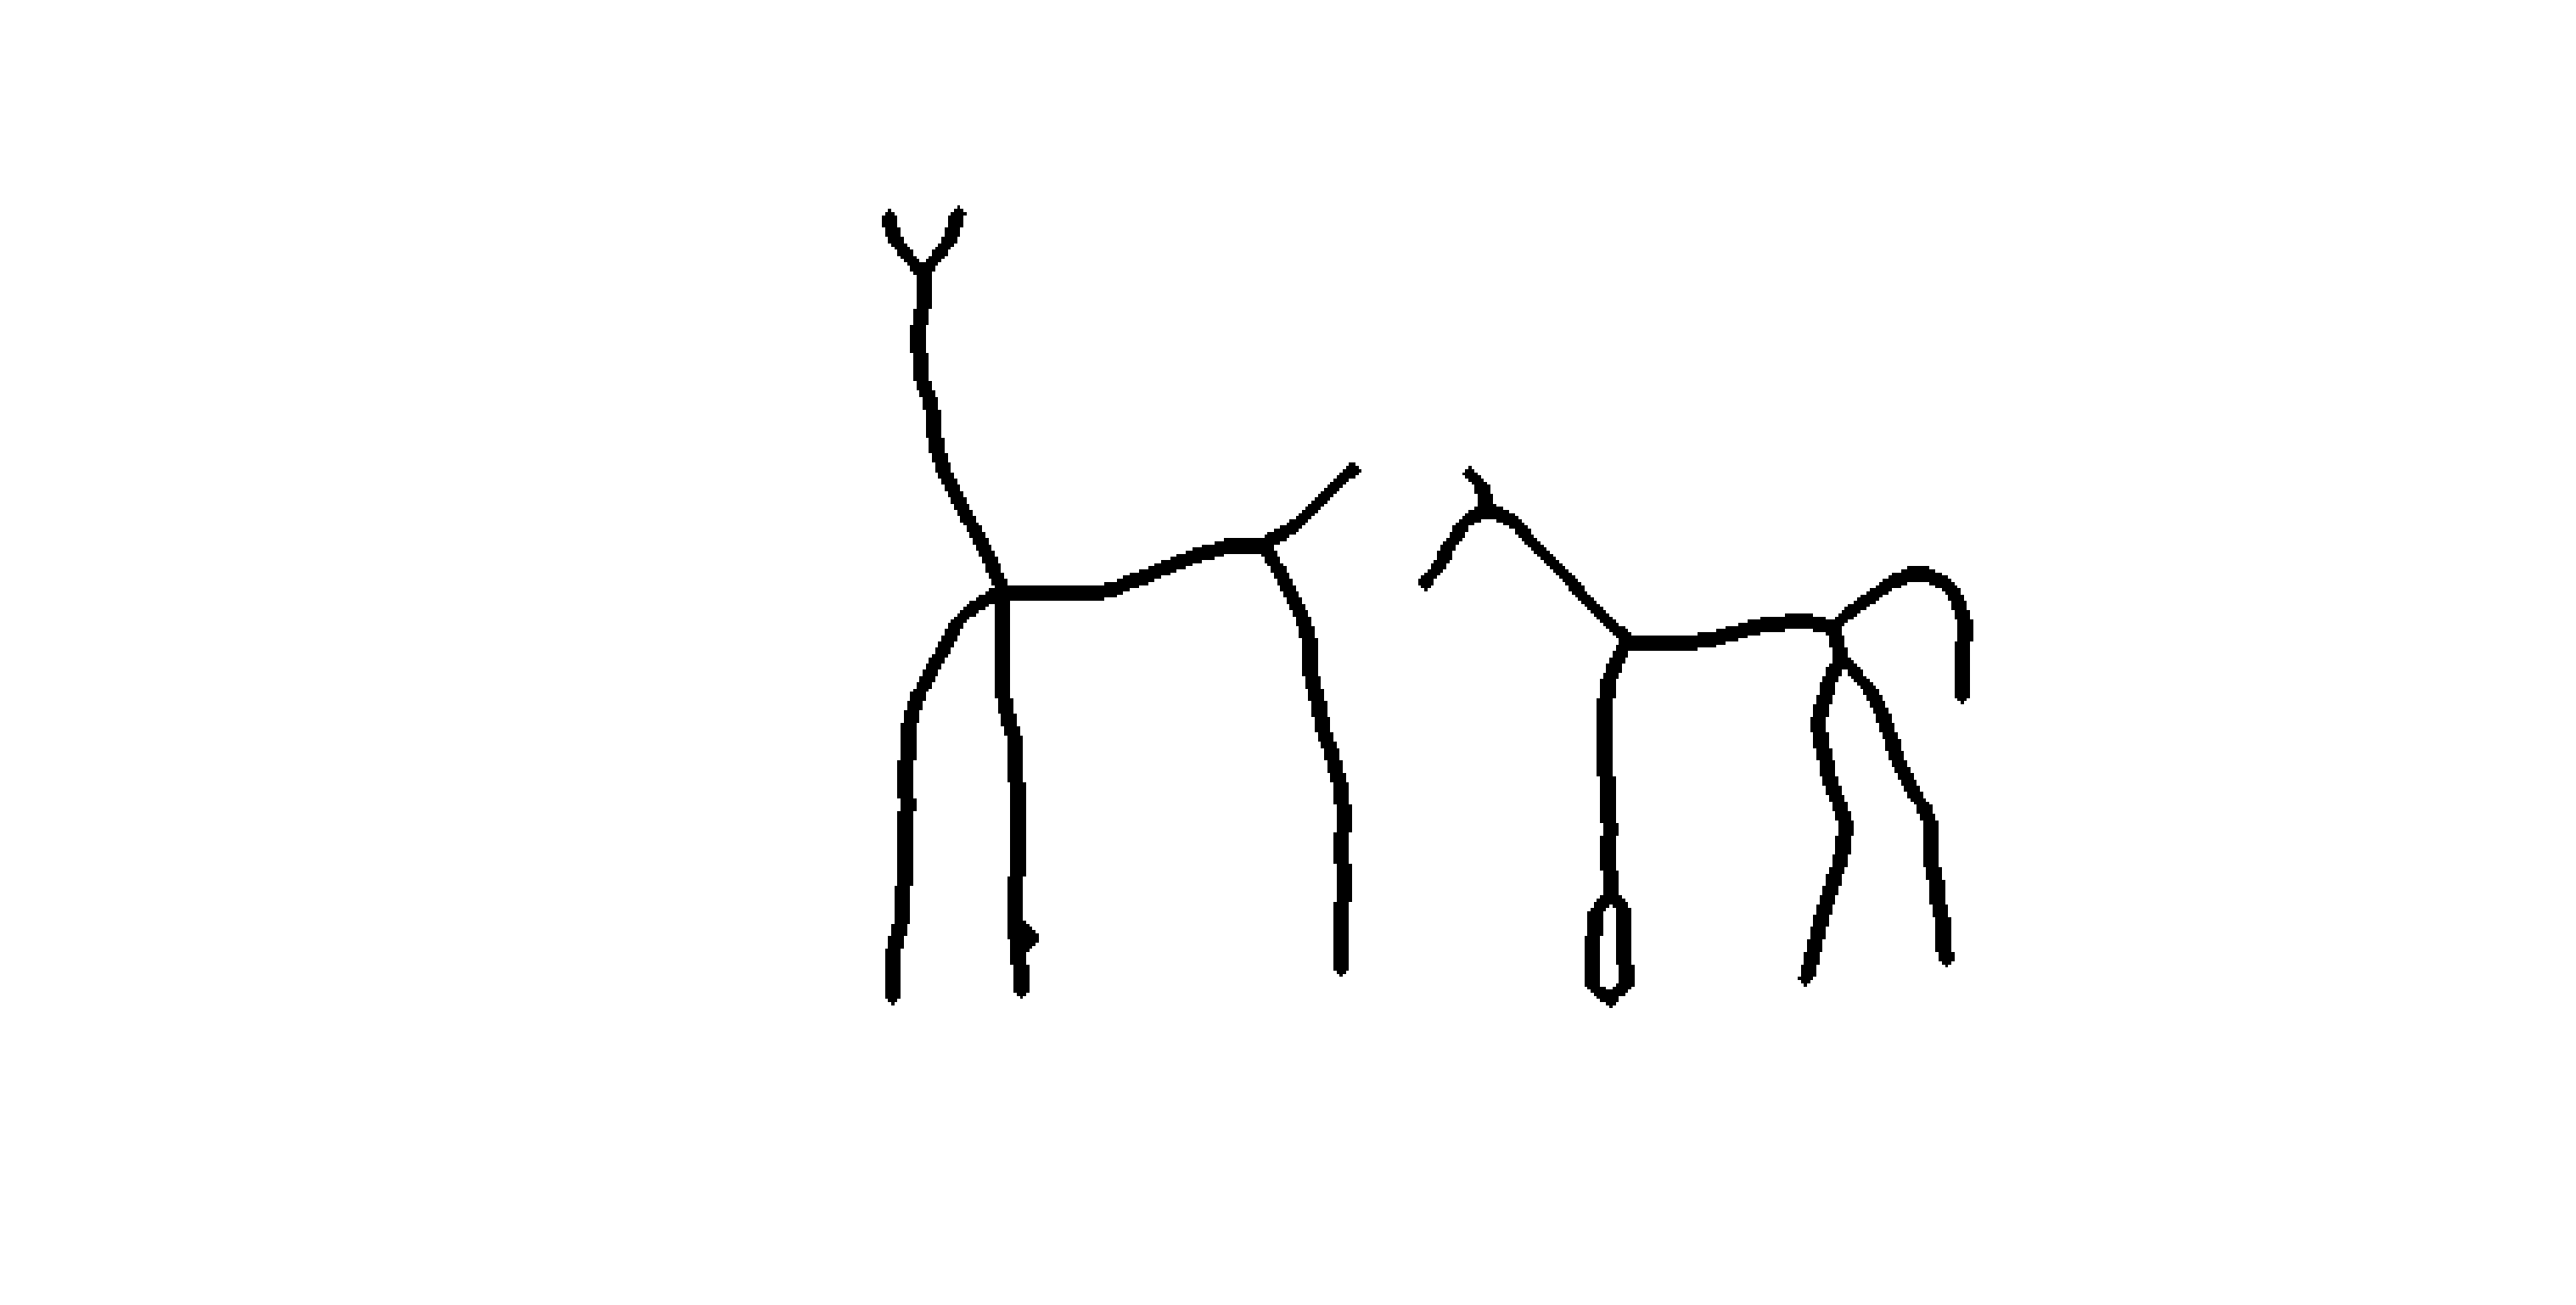
\includegraphics[scale=0.3]{figures/sk_demo1.eps}
\caption{骨架是物体形状的简洁表示,包含了物体的结构信息和物体各部件之间的连接信息。}
\end{figure}

基于骨架的图像中物体表示与识别一直是计算机视觉领域的研究热点。物体的骨架也称作中轴,作为一种物体的形状描述符,
因其同时包含了物体的几何特征(物体各个部分的尺寸大小和角度)和拓扑结构信息(物体各个部件之间的连接关系),
使其在物体识别与表示方面具有独一无二的优势。骨架及相关研究已被广泛应用于基于形状的图像检索
~\cite{demirci2006object,sebastian2004recognition},物体检测和识别~\cite{bai2009active, trinh2011skeleton},
医学图像处理~\cite{sorantin2002spiral},传感器网络分析~\cite{jiang2009case},文字识别~\cite{zhang2015symmetry},
步态识别~\cite{wagg2004automated,tanawongsuwan2001gait}和人体姿态识别~\cite{shotton2013real,girshick2011efficient,sun2012conditional}
等多个研究方向。如何从已分割好的二值图像中提取物体骨架~\cite{saha2016survey}已经取得了很多成果并应用到一些基于形状的物体分类和匹配
~\cite{demirci2006object,sebastian2004recognition,siddiqi1999shock}。但这类算法都是基于已分割好前景和背景的图像,
而如何从自然图像得到分割图像仍是一个待解决的问题。

从自然图像中直接检测物体骨架是一个更具有挑战性的问题,主要有以下几个难点:(1)自然场景的复杂性:自然图像中的场景往往具有复杂的背景,
而这些背景有可能本身具有对称性,比如山峰,草地的倒影,很容易成为误检测点;(2)自然场景中物体的多样性:自然图像中的物体往往呈现多种形态、
颜色、纹理以及形状,例如斑马,鸟类等等;(3)骨架形态的多样性:局部骨架区域具有多种模式,例如T字形,Y字形,各种角度的直线等等。
另外,即使是同一种形态的骨架,由于骨架尺度不一样,他们的局部特征也有很大的差异。

本文的研究目的在于解决骨架提取中尺度未知等难题,完成自然图像中的物体骨架提取,利用提取到的骨架进行图像前景分割以及结合骨架进行候选窗口检测。

\subsection{国内外研究概况}
\subsubsection{自然图像中的物体骨架提取}
近十年来涌现出了很多自然图像中的骨架检测算法,广义上他们可以分为两类:(1)基于传统图像处理的方法~\cite{jang2001pseudo, lindeberg1998edge, yu2004segmentation, zhang2007accurate},
通过计算图像中梯度响应强弱以及边缘和骨架之间的位置关系来定位骨架;(2)随着机器学习技术的兴起以及在计算机视觉中的广泛应用,基于机器学习的方法也被应用到骨架检测中来
~\cite{sie2013detecting, levinshtein2013multiscale, sironi2014multiscale, tsogkas2012learning},对每个像素周围的区域设计基于梯度的多尺度特征,然后通过训练分类器对输入特征进行分类得到图像的骨架图。

由于梯度响应大的像素点位于物体边缘的概率较大,而骨架往往位于两条平行的边缘之间,通过简单的几何运算就能定位骨架。例如Morse等人~\cite{morse1994muitiscale}
采用差分算子作用于高斯平滑后的灰度图像得到边缘响应图,然后对于边缘响应图上的每一点,根据其一定范围内其它点的边缘强度计算中心点的中轴响应(medial response),
中轴响应的峰值即为所求骨架。这一获得边缘强度图的方法也一直为后来研究者所用。Lindeberg~\cite{lindeberg1998edge}对如何选取平滑图像所用的高斯核尺度参数进行
了研究,他提出了自适应尺度参数选取的方法。Jang和Hong~\cite{jang2001pseudo}定义了一个基于边缘强度图的能量方程,通过最小化该能量方程,
迭代计算伪距离变换图(pseudo-distance map)以得到骨架。该伪距离变换图实际上是欧氏距离变换图的变形,它在边缘强度大的地方距离值小,
在边缘强度小的地方距离值大。这种方法产生的骨架会发生偏移,即骨架并不处于中轴位置上。Yu和Bajaj~\cite{yu2004segmentation}提出通过扩散由边缘强度图初始化的梯度向量场得到骨架图来克服骨架偏移的问题 。以上这些方法都是基于边缘强度图,由于边缘强度图本身对局部纹理变化和干扰非常敏感,因此这些方法只能在前景没有太多纹理干扰而且背景非常干净的图像中有效,这种灰度图像和二值图像差别不大,所以在实际中也难得到应用。Adluru等人~\cite{adluru2007contour}
以已知骨架为参考模板,在边缘图中通过粒子滤波的方法搜索与参数模板相似且与边缘段对称的骨架路径,同时完成物体轮廓连接(contour grouping)。
他们的方法不适合形变较大的物体,同时也很依赖边缘检测的结果。Stahl和Wang ~\cite{stahl2008globally}也试图通过连接图像边缘得到对称的闭合物体轮廓,
同时得到物体的对称轴。他们根据轮廓和骨架之间的对称性定义了一种连接损失,并将边缘连接转化为优化该损失函数的凸优化问题进行求解。他们的方法也依赖于边缘检测的性能,而且计算复杂度非常高。Levinstein等人~\cite{levinshtein2013multiscale}提出了利用多尺度超像素(super pixel)的自然图像中轴检测算法。
他们利用相邻超像素之间的颜色和纹理相似性对超像素进行聚类,处于物体同一部分的超像素因纹理和色彩相似而被聚到一起,因此可以得到物体的部分(object parts),然后用椭圆去拟合物体的每一个部分,最后连接这些椭圆的中心得到物体的对称轴。
这种方法得到的对称轴是非常不平滑和不准确的。Trinh和Kimia~\cite{trinh2009category}以同类物体骨架的共同结构为形状模型,得到多种轮廓模板,
并基于轮廓模板在自然图像中对该类物体进行检测。他们的形状模型需要人工针对特定类别的物体生成,因此影响了该方法的实用性。Bai等人~\cite{bai2009active}提出学习
同类物体的骨架得到骨架联合树,并将其作为模板检测自然图像中的物体,但该方法需要预先分割好的二值图像作为训练样本。

基于图像处理的方法难以处理复杂的场景,而且通常计算量巨大;受限于传统机器学习算法以及人工设计特征的性能,基于传统机器学习的方法也不能有效地检
测复杂场景下的物体骨架,而且这种逐像素分类预测的方法也比较耗时。近年来 Tsogkas 等人~\cite{tsogkas2012learning}借鉴基于学习的边缘检测方法~\cite{martin2004learning},计算图像在颜色和纹理亮度上的差异性特征,
通过多示例学习(MIL:multi instance learning)检测自然图像中的物体对称轴。在多示例学习中,若干个示例(instance)组成一个包(bag),只要包中有一个示例为正样本,这个包就被判为正样本。Tsogkas的方法中某像素点
单个尺度的特征为一个示例,不同尺度的特征组成一个包,只要这个包中有一个尺度的特征符被判断为正,那么这个像素点就被认为位于骨架上。
由于该方法并未显式学习特征中的对称性,因此检测的对称轴有时会出现在物体的边缘上,这是因为边缘处的图像特征也具有显著的色彩和纹理差异。
Tsogkas等人的工作中还公布了一个用于训练和评估对称轴检测性能的数据集,该数据集借用用于图像分割的Berkeley300数据集提供的人工分割标注,利用二值图像求骨架的算法得到物体的真实对称轴(ground-truth)。
这个数据集也存在一些缺陷,由于Berkeley300 数据集本身是用于边缘检测和图像分割的,部分图像并没有明确意义的物体,另外Berkeley300数据集中每幅图像由多人标注,不同标注之间存在歧义,因而整个数据集的ground-truth显得很杂乱,有的甚至在物体的边缘处,如图~\ref{fig:sym300} 所示,这对模型训练和识别是十分不利的。
\begin{figure}[htbp]
  \centering
  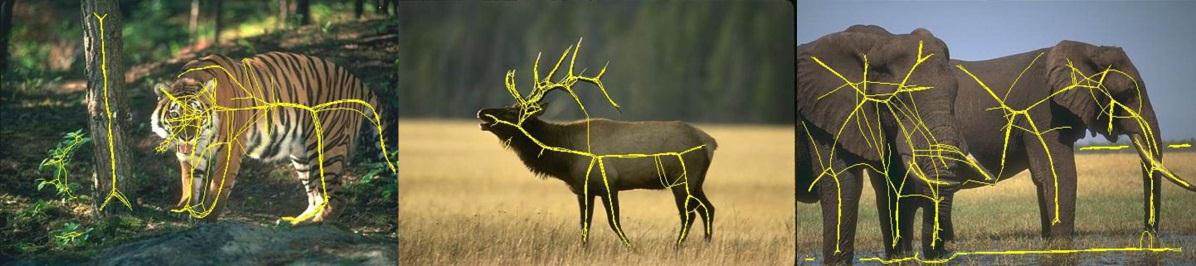
\includegraphics[width=0.8\textwidth]{figures/sym300.png}
  \caption{Tsogkas等人~\cite{tsogkas2012learning}提供的用于自然图像对称轴检测数据集图像样例,中间黄色线条为ground-truth。}\label{fig:sym300}
\end{figure}

\subsubsection{自然图像的前景分割}
图像分割是指根据图像的纹理、色彩、灰度和语义信息将图像分成若干个互不交叠具有独特性质的区域的过程,通常视觉上相似或者语义上相近的像素会被分到同一区域。前景分割是指分割出图像中的物体和人类视觉
感兴趣部分。图像分割是计算机视觉中非常基础的任务,由于它在轮廓检测~\cite{arbelaez2011contour},目标检测~\cite{leibe2008robust},图像中文字区域检测~\cite{chen2004text}中的应用,受到了广泛的关注。

总的来讲图像分割算法分为以下几类:1)基于轮廓的分割方法。轮廓指图像中物体之间的边界,体现了恢复、颜色、纹理等的突变,位于轮廓两侧的像素点不属于一个区域,基于轮廓的分割方法首先通过对图像进行轮廓检测,
然后根据检测出的轮廓分割图像。2)基于区域的方法。这列方法将像素点按照相似性准则分成若干个区域,然后通过逐渐合并、分割区域来进行图像分割。3)基于图论的分割方法。这类方法将图像中的像素作为图论中图(graph)的一个节点,
然后使用min-cut等图(graph)分割方法进行图像分割。
前景指图像中包含物体或者人类视觉注意集中的区域,在图像中物体具体类别未知的情况下从自然图像中区分出前景和背景是人类视觉系统的一项重要的能力。由于图像前景往往是人类视觉感兴趣的区域,这些区域内的物体识别、
检测和分割是计算机视觉研究的重点,前景分割技术被广泛应用于医学扫描图像中的疾病诊断~\cite{pereira2014segmentation},自然图像中的目标检测~\cite{girshick2014rich}。

CPMC~\cite{carreira2010constrained}通过图论中的图分割(graph cut)算法,将图像中互不交叠的小区域作为图(graph)的一个节点,然后使用graph-cut算法将graph分割成若干个子图( subgraph ),形成图像的分割片段。CPMC可以产生
与图像中的物体覆盖率很高的分割片段(图~\ref{fig:seg_skl}和图~\ref{fig:seg_wh}),但是它是基于非监督的方法,算法本身并不能知道产生的分割片段位是前景还是背景,
而且会产生非常多的分割片段(如表~\ref{tb:seg_eval_wh},在WH-SYMMAX数据集上CPMC平均每张图产生511个分割片段)。Shape Sharing也是一种基于图分割的图像分割技术,它利用到了不同类别物体之间会共用一些形状的这一特性,
在分割的时候去寻找数据库中类似的形状并与图像相匹配。FCN~\cite{long2015fully}使用全卷积网络对图像做像素级分类得到语义分割的结果,由于训练时图像标注了类别信息,因此能得到带有具体类别信息的分割结果。通过将FCN分割结果
中的前景类别合并可以得到前景分割的结果,但是训练图像需要逐像素的详细类别标注。

\subsubsection{候选窗口检测}
候选窗口检测(object proposal detection)是一种为目标检测算法提供候选窗口的技术。由于图像中物体大小和形状未知,无法确定合适尺寸和位置的检测窗口,通常目标检测算法依赖于一种称为“滑动窗口”(sliding window)的方法:
通过使用不同大小和比例的窗口在图像上滑动遍历整幅图像,然后在每一个窗口内进行目标检测。显然这种方法是非常低效的,因为一幅图像可能产生成千上万个滑动窗口,在检测之前不知道这些窗口中是否存在目标物体。

有很多研究者想通过降低候选窗口个数的方法解决目标检测的效率问题~\cite{uijlings2013selective, cheng2014bing,zitnick2014edge}。这些方法都会输出大量的候选窗口和窗口对应的似物性得分( objectness score ),表示窗口内
含有物体的可能性。Selective Search~\cite{uijlings2013selective}通过将图像进行超像素分割,然后逐渐合并邻近相似的超像素,直到整张图被合并成一个超像素。由于属于同一个物体的不同超像素在空间上相互邻近,颜色和纹理具有相似性,
因此在合并过程中会率先被合并到同一个超像素里。在超像素合并过程中的每一个合并的超像素都将作为一个候选窗口,训练一个二分类器。在候选窗口提取阶段首先对输入图像进行同样的超像素分割和合并操作,并将合并过程中产生的候选窗口
送入训练好的二分类器得到每一个候选窗口的似物性得分。由于合并超像素过程中产生的候选区域本身就比滑动窗口产生的窗口少,而且经过分类器筛选之后保留的窗口个数更加精简,Selective Search算法能够提供质量优良且数量精简的候选窗口,
但是缺点是超像素分割和合并过程十分耗时,对目标检测来说得不偿失。Bing~\cite{cheng2014bing}利用了物体通常由闭合的轮廓包围这一特性,设计了基于梯度图特征的分类器来检测窗口中的似物性。物体轮廓处通常是梯度响应大的地方,因此梯度图
中的物体会被一圈梯度响应强烈的点所包围,通过梯度图中物体的这种特性,设计一个简单的二分类器即可对每一个窗口进行评分。同时Bing通过对梯度进行量化,将SVM分类器中的乘法和加法转换为比特位操作,加速了候选窗口检测过程,可以以300帧
每秒的速度进行检测。Edge Boxes~\cite{zitnick2014edge}也利用了物体被轮廓所包围这一特性,与Bing不同的是,Edge Boxes通过直接对检测出的轮廓图进行计算得到窗口的得分,而Bing使用的是图像的梯度图。首先Edge Boxes使用
Structure Edge~\cite{dollar2015fast}算法检测图像轮廓,然后将相邻的轮廓点根据轮廓方向合并成轮廓片段,并设计了一些列的规则对候选窗口内的轮廓片段进行打分。例如与候选窗口边界相交的轮廓片段$E_b$得分为0,与$E_b$直接相连的轮廓片段
得分也为0,候选窗口内轮廓片段越长得分越高等等。最后通过计算候选窗口内所有轮廓片段得分的总和作为候选窗口的似物性得分。

\subsection{论文的主要研究内容}
本文的主要研究工作以自然图像中的骨架提取为中心展开,包括骨架提取、基于骨架的前景分割、结合骨架的候选窗口检测和基于骨架提取的对称物体检测。如前文所述,好的表示能够帮助提高识别的性能。而骨架作为一种物体形状和部件连接关系的精简表示,在非刚性物体的识别和检测中具有
独一无二的优势。只有提取的骨架能够有效地表示物体的重要特征,基于骨架的检测和识别算法才能体现出优势。本文着重强调了骨架尺度多变是骨架检测的主要难点之一,针对骨架尺度多变这一特性,设计了尺度相关的side-output网络结构,
在检测骨架的同时能够得到骨架的尺度信息。更进一步,本文利用多任务学习在检测骨架的同时直接预测骨架的真实尺度,在不影响骨架检测性能的情况下能够得到所检测骨架的准确尺度。由于本文提出的模型在检测骨架的同时能够得到骨架的尺度信息,
利用骨架和骨架的尺度信息,通过作以骨架为中心,骨架尺度为半径的圆就可以得到物体的分割。本文所提出的方法可以在不需要任何类别相关信息的情况下,进行图像前景分割。由于目标检测的对象大多位于图像的前景上,可以通过计算检测窗口内部前景
分割的所占比例预测窗口内包含物体的可能性,通过对已有的候选窗口检测算法增加基于前景分割的修正项,极大地抑制了位于图像背景上的候选窗口的似物性得分,提高了候选窗口检测算法的性能。同时本文所提出的骨架检测算法也适用于对称物体的检测,例如航拍图中的道路和自然图像中的文本行等等,因为骨架本身也是一种具有对称性的结构。

\subsubsection{自然图像中的物体骨架检测}
骨架又称中轴,是图像中物体轮廓最大内接圆圆心的集合。由于(1)自然图像中复杂的背景,(2)前景上复杂的纹理,(3)骨架尺度未知,使得从自然图像中提取轮廓异常困难,基于骨架的后续工作也无法有效进行。文献~\cite{sie2013detecting,tsogkas2012learning}
提出通过设计一种多尺度的骨架特征然后用机器学习模型预测图像在多个尺度下的响应,最后结合不同尺度的响应能够解决骨架的尺度问题。但是这种方法会在输出上造成很多噪声,而且受限于所用机器学习模型,
检测出的骨架带有大量假阳点(false positive)。
\begin{figure}[!htb]
  \begin{minipage}[b]{0.7\linewidth}
    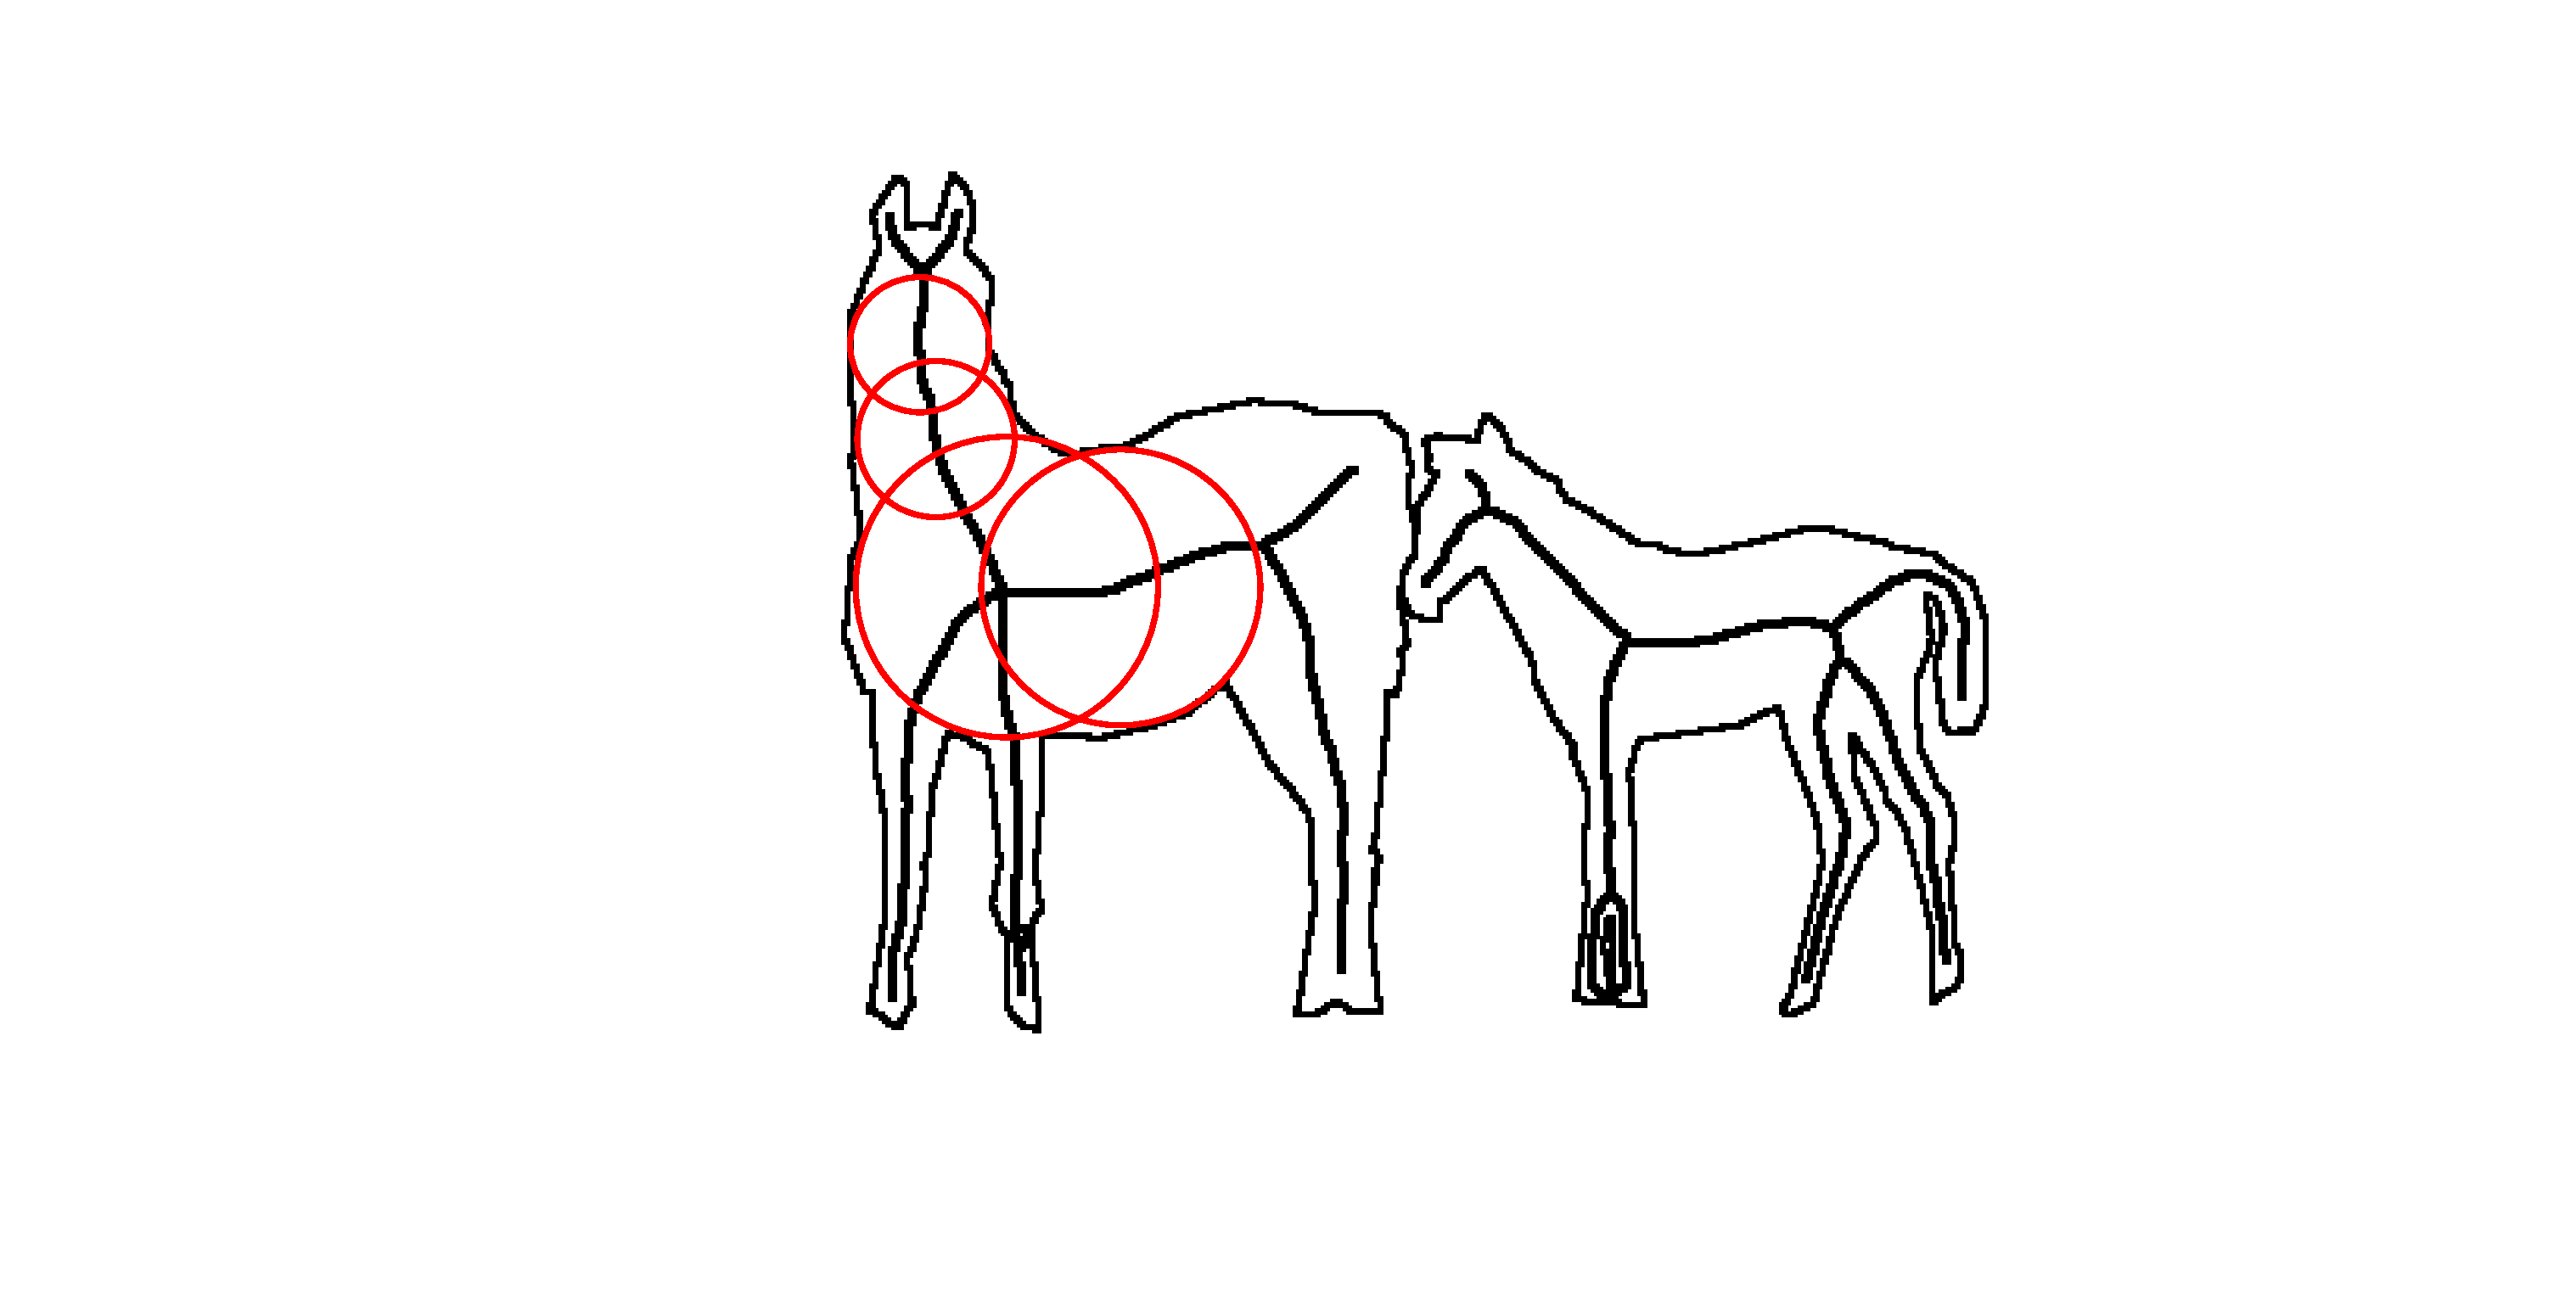
\includegraphics[width=.8\linewidth]{figures/sk_edge}
    \vspace{4ex}
  \end{minipage}%%
  \begin{minipage}[b]{0.5\linewidth}
    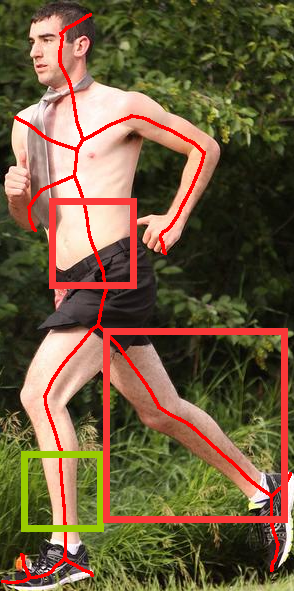
\includegraphics[width=.3\linewidth]{figures/sk_diff_scale_bbox} 
    \vspace{4ex}
  \end{minipage} 
  \caption{左:骨架是物体轮廓最大内接圆圆心的集合;右:骨架尺度多变,只有检测窗口略大于骨架尺度才能有效提取骨架信息。}
  \label{fig:sk_scale_edge}
\end{figure}

神经网络因为具有极强的从数据中学习的能力而被广泛应用于诸多计算机视觉领域~\cite{krizhevsky2012imagenet, newell2016stacked,zhang2014panda,long2015fully}。神经网络强大的学习能力可以从复杂的噪声中学习有用特征表达,
例如Shen~\cite{shen2015deepcontour}利用神经网络学习到的特征替换~\cite{dollar2015fast}中的基于梯度和纹理的特征,取得了更好的轮廓检测的效果。本文设计了一种基于神经网络的多输出骨架检测模型,利用神经网络的学习能力
克服图像中前景和背景复杂的问题。同时卷积神经网络中不同层的神经元具有不同的感受野,利用不同层的side-output检测不同尺度的骨架,解决骨架尺度多变的问题。

\subsubsection{图像中的前景分割}
前景是图像中物体所在的区域,也是人类视觉会率先关注的区域。前景分割是指在图像中具体物体类别未知的情况下分割出图像的前景区域。得到图像中物体的骨架实际上已经知道了物体的位置和结构信息,如果能得到骨架的准确尺度信息,
就可以恢复出物体的区域,实现图像的前景分割。

前文所述具有多尺度side-output的骨架检测算法实际上已经能够获取关于物体骨架尺度的粗略信息,这是因为不同的side-output负责检测不同尺度的骨架,通过计算每个side-output上对同一个像素点骨架的响应,就能得到该点骨架尺度的粗略估计。
但是由于卷积神经网络中各层感受野变化跨度很大,这种方法估计的骨架尺度不准确,特别是对于尺度较大的骨架误差较大,这样会导致恢复出来的前景分割不准确。

为了准确地进行前景分割,就必须准确地估计骨架的尺度。本文在多尺度side-output结构的基础上,设计了多尺度多side-output的\textbf{多任务}网络结构,在检测骨架的同时\textbf{直接估计骨架点的尺度值},在不影响骨架检测性能的同时得到
骨架尺度的精确估计,通过检测到的骨架结合估计的骨架尺度,实现准确地前景分割。

\subsubsection{结合骨架的候选窗口检测}
由于图像中目标的大小、比例和位置未知,一般目标检测依赖于滑动窗口去遍历整个图像,然后在每一个窗口上进行检测,这样做计算代价昂贵。候选窗口检测旨在于为目标检测提供数量精简的候选窗口,这就要求候选窗口检测算法:(1)能够提供尽可
能少的检测窗口,(2)所提供检测窗口尽可能包含图像中的每一个物体,(3)检测窗口的大小和位置尽可能准确。Edge Boxes~\cite{zitnick2014edge}根据\textbf{物体由闭合的轮廓包围}这一假设,根据检测出的物体轮廓为候选窗口评分,输出高分的候选窗口。
由于局部纹理对轮廓检测的结果存在干扰,同时影响了Edge Boxes的结果。显然,利用骨架和骨架恢复出的分割能够抑制图像背景上的候选窗口。本文通过计算前景分割占候选窗口的比例来修正Edge Boxes算法给候选窗口的评分,
抑制了背景上纹理的干扰,提升了Edge Boxes所产生候选窗口的质量。

\subsubsection{基于骨架检测算法的对称性检测}
自然图像中的某些目标具有对称性,例如航拍图中的道路和自然图像中的文本行。可以通过检测这些对称物体的中轴线或者对称轴(axis)来实现对称物体的检测和定位。文献~\cite{sironi2014multiscale}通过回归像素点离中轴点的距离来检测航拍图中道路的中轴线,同时公开了一个航拍图的数据集。在该数据集上的实验结果表明本文所提出的骨架检测算法能取得比~\cite{sironi2014multiscale}更好的道路检测效果。
Zhang~\cite{Zhang15}提出了一种基于对称性的文本行检测算法,该算法利用文本行的对称性提取文字的候选区域。通过使用本文所提出的骨架检测方法替换~\cite{Zhang15}中的对称性检测算法,提升了文本行检测的性能。

\subsection{本文章节安排}
本文围绕自然图像中的骨架提取这一中心,首先阐述本文所提出的骨架提取和骨架尺度预测方法。然后介绍骨架的应用,即利用骨架和尺度恢复物体分割、提取目标检测候选窗口,以及使用骨架提取算法进行对称物体检测。

本文的章节安排如下:

第一章介绍了论文的选题背景,意义,研究思路,当前研究现状以及本文章节安排;

第二章首先介绍了卷积神经网络和全卷积网络,以及几个利用全卷积网络进行图像逐像素预测的例子,并讨论了利用现有技术进行骨架检测将面临的主要困难,以及现有技术的主要缺点;

第三章重点阐述本文所提出的基于尺度相关的边输出(SSO:scale-associated side-output)和多任务网络的骨架检测方法,并分别定量和定性分析了所提出方法相比现有算法的优越性;

第四章介绍了骨架的几个应用:利用所提取的骨架恢复出物体的分割、检测候选窗口,以及在航拍图中进行道路检测和自然场景中文本行检测。

第五章总结全文,并展望未来工作。


%%%%%%%%%%%%%%%%%%%%%%%%%%%%%%%%%%%%%%%%%%%%%%%%%%%%%%%%%%%%%%%%%%%%%%%%%%%%%%%%%%%
%%%%%%%%%%%%%%%%%%%%%%%%%%%%%%%%%%%%%%%%%%%%%%%%%%%%%%%%%%%%%%%%%%%%%%%%%%%%%%%%%%%
\pagebreak
\section{全卷积网络和像素级别的预测}
%\subsection{卷积神经网络}
%神经网络是一种模拟人类大脑的机器学习模型,它的基本单元称为“神经元”(neuron)。如图~\ref{fig:neuron}所示,和大脑中的神经元一样,神经网络中的神经元是一个多输入单输出的结构。
%\begin{figure}[H]
%\centering
%\includegraphics[scale=0.6]{figures/neuron01.png}
%\caption{和人脑神经元(右)一样,神经网络中的神经元(左)也是多输入单输出的结构。}
%\label{fig:neuron}
%\end{figure}
%图~\ref{fig:neuron}中的神经元接收三个输入$x_1, x_2, x_3$,每一个输入都对应一个权重$w$,$w$称为神经元的\textbf{参数}。最终神经元的输出(又称为激活值activation)$a = f(w_1x_1 + w_2x_2 +w_3x_3 + b)$,其中函数$f(\cdot)$称为神经元的\textbf{激活函数},一般是一个非线性的单调函数,比如$\text{sigmoid}(x) = \frac{1}{1+\exp(-x)}$,参数$b$称为神经元的\textbf{偏置}。为了表述方便,我们经常省略偏置,上式中神经元的激活可向量化为$a = W^T \cdot X$。
%
%
%神经网络一般由多层神经元前后连接而成,前层的输出是后层的输入。其中接收数据输入的层称为“输入层”(input layer),输出数据的层称为“输出层”(output layer),其它层称为“隐层”(hidden layer)。我们所说的深度学习,实际上是指\textbf{包含不少于两个隐层的神经网络模型}。图~\ref{fig:nn1}是一个简单的三层神经网络,它的隐层是一个“全连接层”(fully connected layer),因为\textbf{该层的神经元和前层的每一个神经元相连}。
%\begin{figure}[H]
%\centering
%\includegraphics[scale=0.6]{figures/nn1.png}
%\caption{一个简单的三层神经网络,中间层的神经元和前层(输入层)的每一个神经元相连,这样的层被称为“全连接层”。}
%\label{fig:nn1}
%\end{figure}
%我们用$w_{ji}^{(l)}$表示“第$l$层的第$i$个神经元和第$l+1$层的第$j$个神经元之间的权重”,那么图~\ref{fig:nn1}中的神经网络中隐层(第二层)第一个神经元的激活值为$a^{(2)}_1 = f(w_{11}^{(1)}x_1+w_{12}^{(1)}x_2+w_{13}^{(1)}x_3 +b)$,最终网络的输出$a^{(3)}_1 = f(a^{(2)}_1w^{(2)}_{11}+a^{(2)}_2w^{(2)}_{12} + a^{(2)}_3 w^{(2)}_{13})$
%
%
%卷积神经网络最早由Lecun发明并应用到手写数字识别中~\cite{lecun1998gradient},2012年Hinton等人使用7层的卷积神经网络~\cite{krizhevsky2012imagenet}在ImageNet图像分类中取得了历史性的突破,将错误率从25.8\%降低到了16.4\%,引领了深度学习的热潮。从此之后基于深度学习(深度卷积神经网络)的方法占领了计算机视觉几乎所有的领域,不论是底层(low level)的图像分割~\cite{long2015fully,noh2015learning}、图像轮廓检测~\cite{xie2015holistically,shen2015deepcontour},还是高层(high level)的图像分类~\cite{krizhevsky2012imagenet,he2016deep},人体姿态估计~\cite{zhang2014panda,newell2016stacked}等等,深度学习在这些任务上都取得了远优于传统方法的结果。
%
%卷积神经网络主要由若干个卷积层(convolution layer)、池化层(pooling layer)和全连接层(fully connected layer)组成。首先经过若干个卷积层和池化层对图像进行特征提取(feature extraction),输出保留了空间信息的特征图(feature map),然后使用若干个全连接层对特征图进行特征映射,得到不包含空间信息的特征向量,最后使用这个特征向量进行后续的识别和检测。
%
%\subsubsection{卷积特征提取}
%\textbf{卷积层}是卷积神经网络中最重要的一种操作(opterator)。图像中的信息具有很强的空间相关性,同时图像中的特征也有位移不变性,例如目标物体在图像上方或者下方并不会影响图像的语义,这也就意味着在图像中某个位置学到的特征在另一个位置同样适用。
%
%卷积就是一种具有位移不变性的操作。通过使用固定大小的卷积核(kernel)在图像上以一定步长(stride)滑动,并在每一个位置计算卷积核与图像的内积作为该位置的输出。图~\ref{fig:conv1d}是一维空间上卷积的例子,一个3维的卷积核在长度为6的输入上卷积,卷积核每次移动的步长为1,移动三次(不包含第一次)得到长度为4的输出。
%\begin{figure}[H]
%\centering
%\includegraphics[scale=0.4]{figures/conv1d.png}
%\caption{大小为3的一维卷积核在长度为6的输入上卷积,得到长度为4的输出。}
%\label{fig:conv1d}
%\end{figure}
%
%由于图像是二维信号(考虑到图像通道实际上是三维,但通常我们只考虑图像的空间平面而忽略通道),卷积神经网络中的卷积核一般是二维的。例如图~\ref{fig:conv2d}使用一个$2 \times 2$的卷积核作用到$5 \times 5$的输入上,得到$4 \times 4$的输出矩阵。在卷积神经网络中,这样的一个卷积核实际上代表着一个神经元,卷积核的大小表示神经元输入的个数,卷积核的值表示神经元对各输入的权重。通常卷积神经网络中的一层包含着若干个大小相同但权重各异的卷积核,假设某一层有$c$个卷积核,每个卷积核的输出大小为$w \times h$,那么该层最终输出的\textbf{特征图}(feature map)的形状就是$w \times h \times c$。正如前文所述,考虑到输入图像和中间层输出的通道数,实际上卷积神经网络中的卷积核是三维的,为了表述方便,我们通常忽略只考虑空间平面,从而把它简化为二维操作。
%\begin{figure}[H]
%\centering
%\includegraphics[scale=0.5]{figures/conv2d.png}
%\caption{二维卷积:大小为$2\times2$的卷积核作用到$5\times5$的输入上,得到$4\times4$的输出。}
%\label{fig:conv2d}
%\end{figure}
%
%总的来说,卷积操作可以在显著减少神经网络参数的同时带来位移不变性等适合图像信号的特性,使得卷积神经网络在计算机视觉中得到了广泛应用。想象我们有一个$500\times500\times3$的输入数据,后一层有100个神经元,如果使用全连接层,那么该层将有$500\times500\times3\times100=75,000,000$个参数,而如果使用卷积核大小为$3\times3$的卷积层,那么参数个数将减少到$3\times3\times3\times100 = 2700$个。
%
%\subsubsection{池化和特征汇聚}
%在通过卷积得到特征(feature)之后,我们就要用这些特征进行识别。理论上讲,我们可以使用提取到的所有特征去训练检测器,例如softmax或者SVM等分类模型。但是这样面临着巨大的计算量的挑战。上一节中的例子,假如我们用100个$3\times3$的卷积核作用到$500\times500\times3$的输入上,将会得到$498\times498\times100$

\subsection{全卷积网络(FCN)和图像语义分割}
全卷积网络(FCN:Fully Convolutional Networks)由Long等人~\cite{long2015fully}提出并应用在图像的语义分割上。由于全卷积网络能够高效地进行像素级别的预测(pixel-wise prediction)因此被广泛应用于轮廓检测
~\cite{xie2015holistically,liu2016richer},人体姿态估计~\cite{bulat2016human,newell2016stacked},图像显著性检测~\cite{wang2016saliency}等任务中。这些任务有一个共同点,那就是需要进行“像素级的预测”。
以图像中物体轮廓检测为例,轮廓检测需要预测图像中每一个像素位于物体轮廓上的可能性。

受限于传统的机器学习模型,这种需要像素级预测的任务往往采用以某个像素为中心提取特征然后逐像素预测的方式。例如~\cite{shen2015deepcontour}使用深度卷积网络提取某像素为中心的图像块特征,然后输入
到~\cite{dollar2015fast}中的structure forest,预测图像块中心像素位于轮廓上的概率,然后将每个像素的预测结果拼接成轮廓检测结果。受限于所取图像块的大小,这类方法不能够提取图像中的全局特征;而且图像块之间存在相当多
的重叠(overlap),计算冗余度很大。

全卷积网络使用全卷积层(fully convolution)代替卷积神经网络中的全连接层,得到逐像素的表示,并使用反卷积层(deconvolution)将输出特征图上采样到和输入图像同样的尺寸,实现逐像素预测。图~\ref{fig:long_fcn}是~\cite{long2015fully}中所
使用的FCN结构。FCN中所使用的反卷积层实际上是一个双线性插值的上采样操作,目的是把经过多次池化( pooling )后分辨率下降的特征图上采样到和输入图像一样的空间尺度上,在训练过程中反卷积层的卷积核处于固定状态,不参与训练。
经过上采样之后得到的预测值再与人工标注的ground-truth逐像素计算损失,然后利用反向传导( back-propagation )和梯度下降(gradient descent)算法更新网络参数,训练神经网络。

\begin{figure}[!htb]
\centering
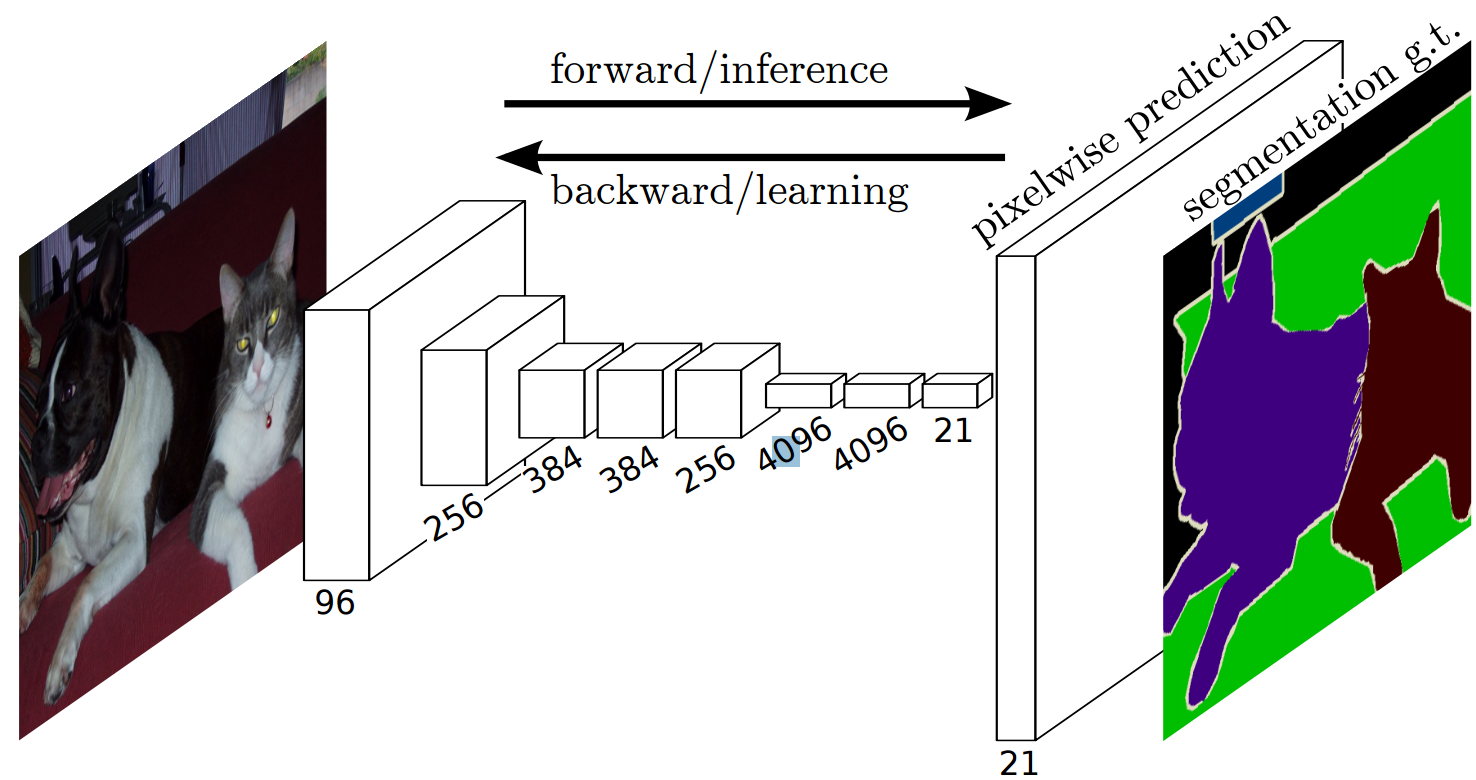
\includegraphics[scale=0.2]{figures/fcn_arch.png}
\caption{全卷积网络的结构:通过使用上采样得到像素级预测(pixel-wise prediction),图像来自~\cite{long2015fully}。}
\label{fig:long_fcn}
\end{figure}

由于~\cite{long2015fully}中的FCN结构使用一个单独的反卷积实现上采样,上采样倍率达到32 (因为FCN网络中含有5个步长为2的池化层),使得最后预测结果在分割边界上比较粗糙。Noh等人~\cite{noh2015learning}设计了一种利用反池化
层(unpooling)进行逐层上采样的网络结构提升预测的精度。图~\ref{fig:noh_deconv}是Noh所使用的网络结构,与~\cite{long2015fully}中的网络不同,这里的上采样操作是逐次使用反池化层完成的,每次的上采样倍率为2。
\begin{figure}[!htb]
\centering
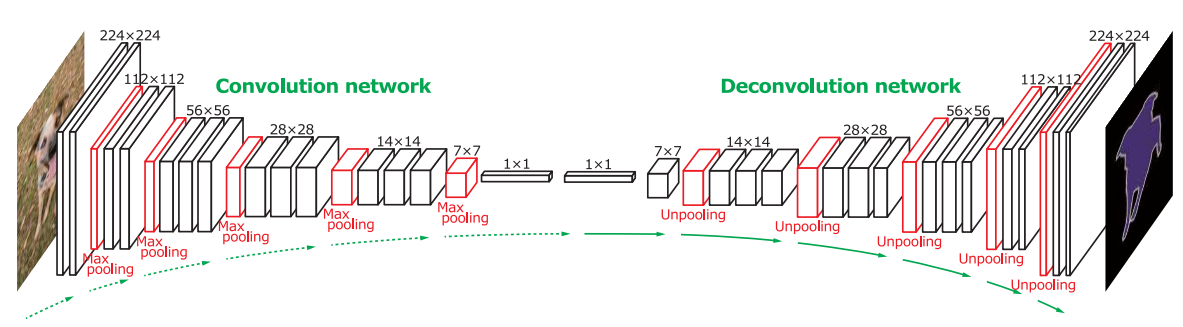
\includegraphics[scale=0.35]{figures/deconv_arch.png}
\caption{~\cite{noh2015learning}所采用的网络结构,通过逐层上采样弥补反卷积带来的分辨率不足问题。}
\label{fig:noh_deconv}
\end{figure}

\subsection{HED图像轮廓检测}
图像中的物体轮廓是指物体与物体或者是物体与背景之间的分界,轮廓检测是计算机视觉中一个被长期研究的热点问题。研究表明,在卷积神经网络中不同的层能学习到不同语义层次的特征,浅层更多的学到局部纹理特征,
中层含有更多的形状、线条等初级语义特征,而深层会学到关于物体、类别等高级抽象的特征。轮廓检测是一个需要同时兼顾低层纹理以及高层语义特征的过程,因为物体内部存在许多亮度变化,这些亮度变化很容易被误检测为轮廓,高层语义特征
能够避免这种误检测(见图~\ref{fig:hed_arch}side-output5),但是高层特征对轮廓定位不准确(图~\ref{fig:hed_arch}side-output5)。由于卷积神经网络中不同的层在输入图像上的感受野大小不一样,因此可以利用中间层输出side-output,这些
感受野不同的side-output可以作为多尺度的检测器。HED(Holistically-nested Edge Detection)~\cite{xie2015holistically}利用多输出结构进行边缘检测。HED以VGG16~\cite{Simonyan14c}网络为基础,在每一个池化层之前的卷积
层(conv1\_2, conv2\_2, conv3\_3, conv4\_3, conv5\_3)输出 side-output ,这5个 side-output 的感受野分别是4、14、40、92、196。在训练阶段,五个side-output都以人工标注的轮廓图为ground-truth分别计算损失,然后各自进行反向传导。
HED的结构并不是传统卷积神经网络的直线型结构,存在一些有分叉的层,例如 conv1\_2 不仅连接了 side-output2,还与后面的 conv3\_1 相连接,这些层在反向传导时梯度等于后续层传回的梯度的和。
\begin{figure}[!htb]
\centering
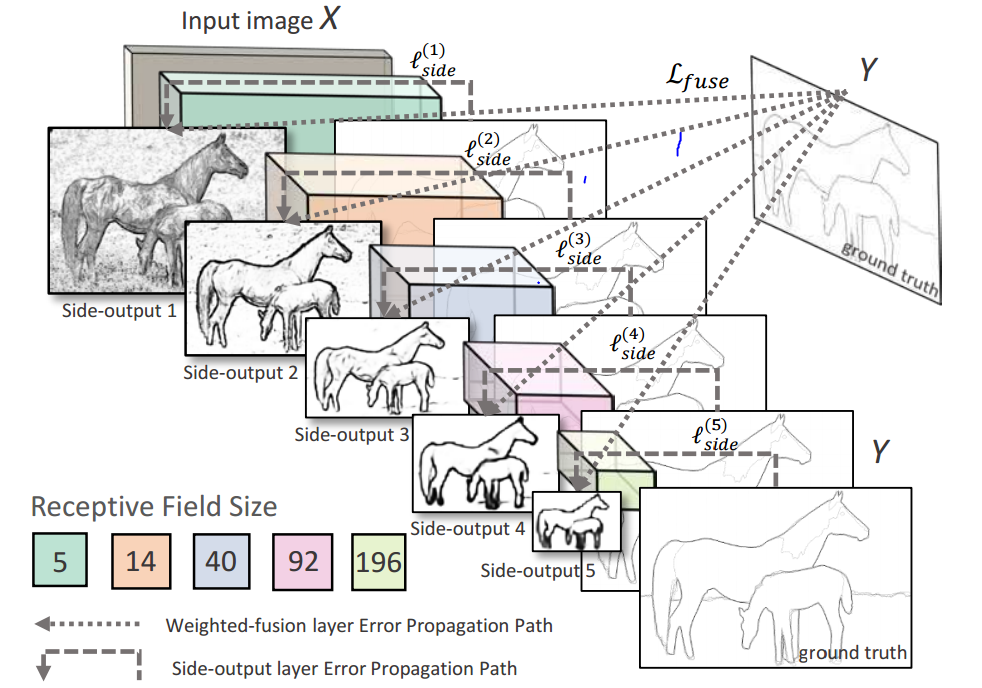
\includegraphics[scale=0.35]{figures/hed_arch.png}
\caption{HED的网络结构,图像来自~\cite{xie2015holistically}。
}
\label{fig:hed_arch}
\end{figure}
图~\ref{fig:hed_arch}是HED的网络结构,side-output1$\sim$side-output5感受野依次增大,但分辨率逐渐减小,这是由于网络中池化层下采样造成的。由于感受野的差异,接近输入图像的 side-output 感受野小,能更多地提取图像局部的
纹理;后面的side-output感受野大,能提取高层语义。最后这五个 side-output 被融合成输出$Y$。

与轮廓检测类似,骨架检测也需要对输入图像的每一个像素进行预测。但骨架检测面临一个新的难题,那就是\textbf{骨架的尺度未知}。与轮廓检测不同,骨架检测必须用合适大小的检测窗口才能提取有效的表示特征。对轮廓检测而言,
检测窗口大小会影响提取的表示特征是否包含足够的上下文信息( context );但对骨架检测而言,检测窗口大小会直接决定\textbf{能否根据窗口中的信息提取到骨架}。图~\ref{fig:edge_vs_sk}用不同颜色的线条表示骨架和轮廓的ground-truth,
线条上的方框表示不同尺寸的检测窗口。对于轮廓检测而言,检测窗口大小的变化并不会对所提取的信息有根本改变,但是对骨架检测来说,不合适的检测窗口尺寸根本就无法提取到有用信息。例如图中红颜色的小方框,虽然方框中心点像素位
于长颈鹿的骨架点上,但是显然仅仅根据这个方框内的信息我们无法判断中心点是否为骨架。
\begin{figure}[H]
\centering
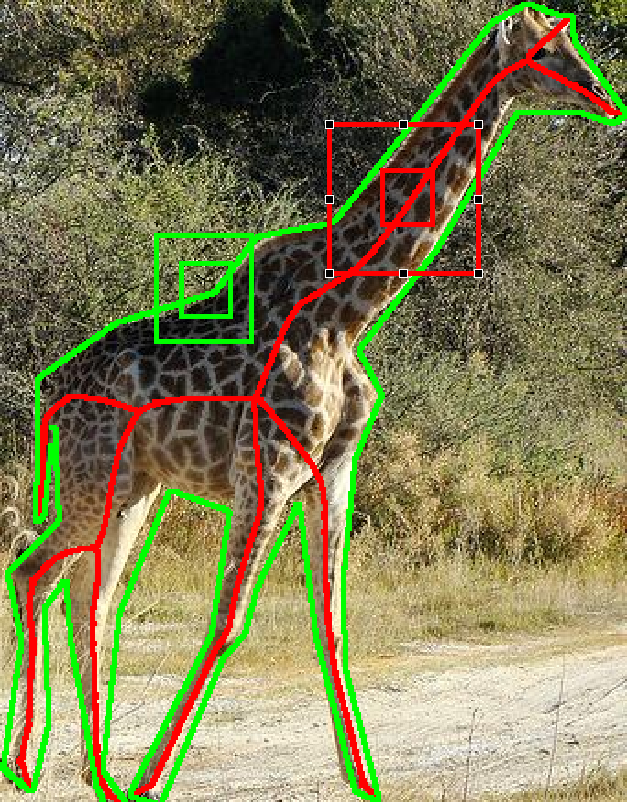
\includegraphics[scale=0.3]{figures/edge_vs_sk.png}
\caption{检测窗口的大小影响骨架检测的结果,只有窗口略大于骨架尺度才能提取有效信息。
}
\label{fig:edge_vs_sk}
\end{figure}
\subsection{本章小结}
本章介绍了利用全卷积神经网络(FCN)进行像素级分类的两个工作。全卷积网络通过用全卷积层替换全连接层,得到了像素级别的图像表示,实现了端到端的像素级预测。

%%%%%%%%%%%%%%%%%%%%%%%%%%%%%%%%%%%%%%%%%%%%%%%%%%%%%%%%%%%%%%%%%%%%%%%%%%%%%%%%%%%
%%%%%%%%%%%%%%%%%%%%%%%%%%%%%%%%%%%%%%%%%%%%%%%%%%%%%%%%%%%%%%%%%%%%%%%%%%%%%%%%%%%
\pagebreak
\section{基于全卷积多输出网络的骨架检测}
在这一章我们介绍本文所提出的骨架检测和骨架尺度预测方法。首先,我们介绍本文所使用的基于HED~\cite{xie2015holistically}的网络结构,然后讨论如何优化和融合本文所提出的融合尺度相关的边输出(scale-associated side-output)多任
务网络来检测骨架和预测骨架尺度。骨架检测是一个分类问题,而骨架尺度预测是一个回归问题,本文提出的多任务网络可在一个框架下将两个任务同时进行。

在HED中,多个side-output均使用同样的人工标注轮廓图作为ground-truth,这是因为用不同尺度的检测窗口检测物体轮廓都会有响应,轮廓检测不存在尺度问题。但是在骨架检测中,我们面临着骨架尺度未知的难题。假若我们也采用HED的结构,
所有的side-output使用同样的ground-truth,那么相当于认为感受野等于4的 side-output1 具备检测所有尺度骨架的能力,这显然是不合理的。正如前文所述,只有检测窗口略大于骨架尺度才能提取到有效的特征进行后续的检测。基于以上分析,
本文提出了尺度相关的边输出(SSO:scale-associated side-output)的概念,根据side-output感受野的不同,输出不同尺度的骨架图。

\subsection{网络结构}
为了克服骨架检测中的尺度问题,我们设计了包含若干个尺度相关的边输出 (SSO: scale-associated side-output )的网络,在训练阶段根据side-output的感受野来确定其 ground-truth。HED网络以VGG16~\cite{Simonyan14c}为基础,并在每组
卷积的最后( conv1\_2, conv2\_2, conv3\_3, conv4\_3, conv5\_3 )使用$1 \times 1$的卷积核输出side-output。在HED网络的基础上,本文做了如下修改:(a)去掉了side-output1,因为其感受野太小,不适合检测任何尺度的骨架,并用尺度
相关的边输出(SSO: scale-associated side-output) 代替side-output;(b)每一个SSO输出若干个尺度相关的骨架图( skeleton map ),不同SSO产生的同一个尺度的骨架图将会用一个尺度相关的权重加权平均,取平均之后的结果作为该尺度的
骨架图,这么做的原因是不同SSO由于感受野不同,对不同尺度的骨架检测结果的置信度有差异,比如底层的SSO对小尺度骨架检测更为精准,而高层SSO对大尺度骨架检测效果更好。这个加权平均过程可以用一个$1 \times 1$的卷积层实现,这样
不同尺度的骨架图将用不同的权重进行融合;(c)每个SSO多出一个用于预测骨架尺度的分支ScalePred-SSO,该分支用一个回归模型估计骨架尺度。图~\ref{fig:lmsds_arch}是本文所提出方法的网络结构图。
\begin{figure}[!htb]
\centering
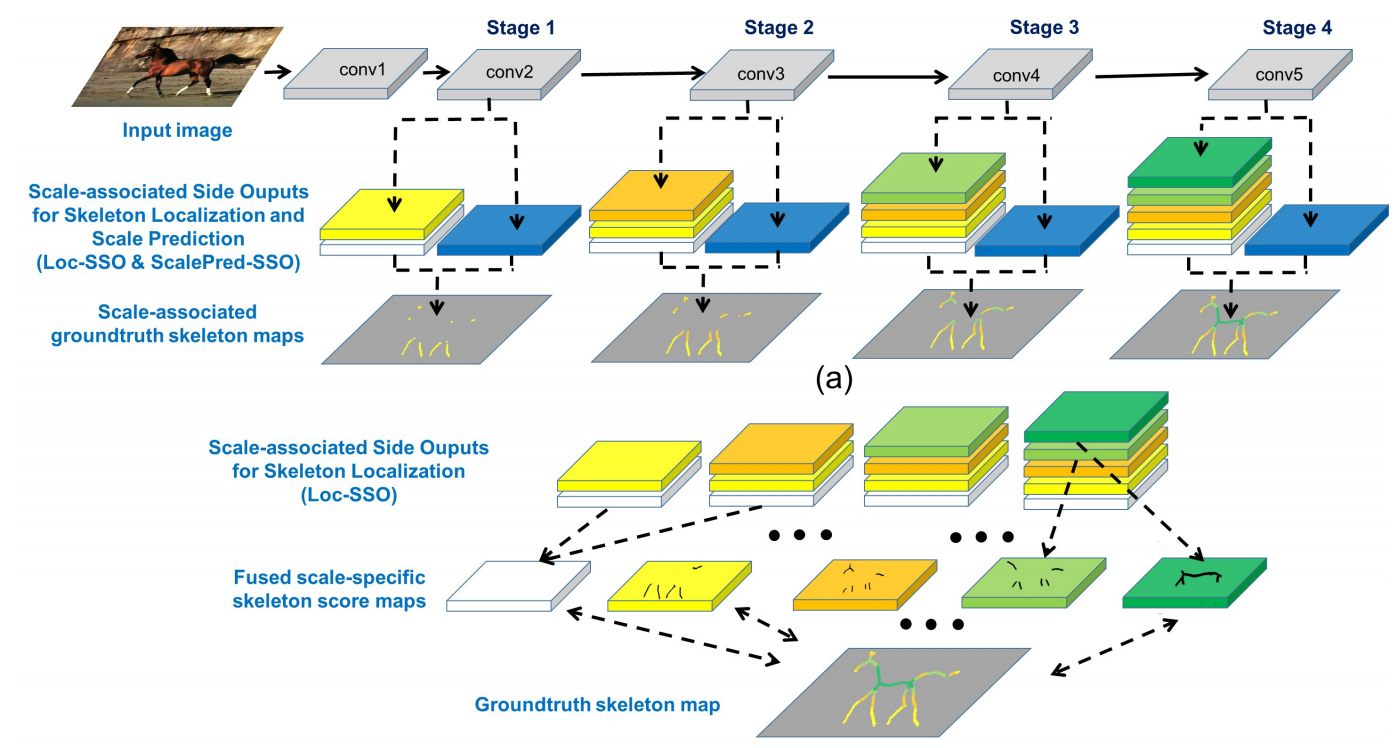
\includegraphics[scale=0.3]{figures/lmsds_arch.png}
\caption{本文所提出多任务多尺度相关边输出网络的结构。图中第二靠右的四个方块表示ScalePred-SSO,左侧是尺度相关的边输出(SSO:Scale-associated side-output),不同SSO感受野不同,输出的尺度相关的骨架图个数也不一样。
}
\label{fig:lmsds_arch}
\end{figure}
图~\ref{fig:lmsds_arch}第一排为VGG16~\cite{Simonyan14c}网络。第二排:在stage1$\sim$4分别加上了两个输出,SSO和ScalePred-SSO,其中左侧多层为SSO,右侧蓝色单层为ScalePred-SSO。
\subsection{通过融合SSO进行骨架检测和尺度预测}
骨架检测可以被表述为一个逐像素的二分类问题,给定输入图像$X=\{x_j, j=1,...,|X|\}$,骨架检测的目的是预测对应的骨架图(skeleton map)$\hat{Y}=\{\hat{y_j},j=1,...,|X|\}$,其中$\hat{y_j} \in \{0,1\}$表示每一个像素点的预测值,
比如像素点$x_j$被预测为骨架,则$\hat{y_j} = 1$,否则$\hat{y_j} = 0$。接下来,我们介绍如何在训练阶段学习和融合尺度相关的边输出(scale-associated side-output)并在测试阶段使用学到的网络参数进行骨架检测。

\subsubsection{多任务多输出网络的训练}\label{sec:train_net}
假设我们有训练数据集 $\mathcal{S} = \big\{\big(X^{(n)},Y^{(n)}\big),n=1,...,N\big\}$ ,其中 $X^{(n)}=\big\{ x^{(n)}_j, j=1,...,|X^{(n)}| \big\}$ 是原始的输入图片,
$Y^{(n)}=\big\{ y^{(n)}_j, j=1,...,|Y^{(n)}| \big\}\big(y^{(n)}_j \in {0,1}\big)$是对应的骨架图。首先我们介绍如何计算每一个训练样本量化的骨架尺度图,在训练的时候将用这些量化的骨架尺度图作为监督。

\vspace{1em}
\noindent \textbf{a)骨架尺度量化}


首先我们定义骨架的尺度为\textbf{以骨架点为圆心的物体轮廓最大内接圆的半径},这可以近似的通过计算骨架点与离骨架点最近的轮廓点之间的距离得到,同时对所有的非骨架点,其尺度为0。这样,我们得到了一个新的骨架
尺度图$S^{(n)} = \big\{s^{(n)}_j,j=1,...,|X^{(n)}|\big\}$,对骨架图$Y^{(n)}$有$y^{(n)}_j = 1(s^{(n)}_j > 0)$,式中$1(\cdot)$是示性函数,括号内不等式成立为1,否则为0。由于我们将整幅图像当做一个整体进行预测,
在之后的表述中将忽略上标$n$。我们的目的是训练一个输出多个 SSO 的卷积神经网络,假设这个网络输出$M$个SSO,这$M$个 SSO 的感受野依次递增,记这些SSO的感受野为$r_i;i=1,...,M$。需要注意的是,\textbf{只有感受野略大于
骨架尺度的卷积层才能够提取有效特征},因此我们可以根据这$M$个 SSO 的感受野对骨架进行量化,表示该骨架点能够被哪一个SSO所检测到(这里我们假设$r_M$足够大,能够检测数据集中所有的骨架点)。骨架尺度$s$量化后的值$z$为:
\begin{equation}
z = 
\begin{cases}
\underset{i=1,...,M}{\arg\max i} \ , \text{s.t.} \ r_i > \lambda s, \text{if} \  s>0 \\
0, \text{if} \ s = 0\\
\end{cases}
\end{equation}
上式中$\lambda > 1$是一个用来保证感受野略大于骨架尺度的系数(在我们的试验中$\lambda = 1.2$)。现在,对一幅图像$X$我们有其量化的骨架尺度图$Z = \big\{z_j,j=1,...,|X|\big\}(z_j \in {0,1,...,M})$。

\vspace{1em}
\noindent \textbf{b)学习尺度相关的边输出(learning scale-associated side-output)}


图像的骨架图$Y$可以由量化尺度图$Z$得到:$Y=1(Z>0)$,但是反之却不行。换句话说,量化尺度图比骨架图含有更多的信息,因此我们用$Z$而不是$Y$去训练神经网络。实际上这将一个二分类问题转化为了多分类问题,
其中每一个类别代表一种量化尺度。正如前文所述,一个SSO只能检测出尺度略小于其感受野的骨架点,这正是SSO(scale-associated side-output)尺度相关的边输出的由来。对于第$i$个SSO:$Z^{(i)} = Z \circ 1(Z<=i)$,$\circ$是
矩阵点乘。假设$K^{(i)}$表示$Z^{(i)}$的最大值,那么$Z^{(i)} = \big\{z^{(i)}_j, j=1,...,|X|\big\},z^{(i)}_j \in \big\{0,1,...,K^{(i)}\big\}$。我们用 $l^{(i)}_s(W, \Phi^{(i)})$ 表示第$i$个SSO的损失函数,
$W$是神经网络的参数,$\Phi^{(i)}$是该SSO分类器的参数。由于我们在整张图像上进行预测,因此损失函数将在训练图像和对应ground-truth的所有像素上计算。通常图像中不同量化类别的骨架点和背景点之间的分布是不均的,
这种不均会对训练造成影响。比如,图像中的大部分点都是背景点,这样训练的模型会在测试阶段认为所有的点都是背景。因此我们定义了一个加权的"softmax"损失函数:
\begin{equation}
l^{(i)}_{cls}(\mathbf{W}, \mathbf{\Phi}^{(i)}) = - \frac{1}{|X|} \sum_{j=1}^{|X|} \sum_{k=0}^{K^{(i)}}\beta^{(i)}_k1(z^{(i)}_j=k)\log \text{Pr}(z^{(i)}_j=k|X;\mathbf{W},\mathbf{\Phi}^{(i)})
\label{eq:weighted_softmax}
\end{equation}

式~\ref{eq:weighted_softmax}中$l^{(i)}_{cls}$是第$i$个SSO的分类损失,下标$cls$表示这是一个分类器的损失函数 (classification),$\beta^{(i)}_k$是第$k$类样本的权重,$Pr(z^{(i)}_j=k|X;W,\Phi^{(i)}) \in [0,1]$是SSO分类器
预测的值,表示像素点$x_j$属于类别$k$的可能性,其中 $\sum_{k=0}^{K^{(i)}}\text{Pr}(z^{(i)}_j=k|X;W,\\ \Phi^{(i)}) = 1$ 。用$\mathcal{N}(\cdot)$表示一个集合中非零点的个数,那么$\beta_k$通过下式计算得到:
\begin{equation}
\beta^{(i)}_k = \frac{\frac{1}{\mathcal{N}(1(Z_i==k))}}{\sum_{k=0}^{K^{(i)}}\frac{1}{\mathcal{N}(1(Z_i==k))}}
\label{eq:beta}
\end{equation}

从式~\ref{eq:beta}可以看出,当第$i$个SSO的ground-truth中属于某个类别$k$的像素点个数 $\mathcal{N}(1(Z_i==k))$ 比较少,那么这个类别上的误判产生的损失将会被施加比较大的权重$\beta_k$,权重$\beta_k$可以一定程度上修正
由于训练样本类别间不均衡带来的影响。

假设$a^{(i)}_{jk}$表示第$i$个SSO对像素点$x_j$在第$k$个量化类别的预测(在神经网络中,神经元的输出被称为激活值activation),那么使用softmax函数$\sigma(\cdot)$来计算
\begin{equation}
\text{Pr}(z^{(i)}_j=k|X;W,\Phi^{(i)}) = \sigma(a^{(i)}_{jk})=\frac{\exp(a^{(i)}_{jk})}{\sum_{k=0}^{K{(i)}} \exp(a^{(i)}_{jk})}
\end{equation}
损失函数$l(W,\Phi^{(i)})$对激活值$a^{(i)}_{jl}(l \in {0,1,...,K^{(i)}})$等于:
\begin{equation}
\frac{\partial l^{(i)}_s(W,\Phi)}{\partial a^{(i)}_{jl}} = -\frac{1}{m}\bigg(\beta^{(i)}_l1(z^{(i)}_j=l)-\sum_{k=0}^{K^{(i)}}\beta^{(i)}_k1(z^{(i)}_j=k)\text{Pr}(z^{(i)}_j=l|X;\mathbf{W},\mathbf{\Phi}^{(i)})\bigg)
\label{eq:partial}
\end{equation}
$\Phi=\big(\Phi^{(i)};i=1,...,M\big)$表示所有SSO的分类器参数。

%,最后所有SSO的损失函数等于各自损失的和:
%\begin{equation}
%\mathcal{L}_{cls}(W,\Phi) = \sum_{i=1}^Ml^{(i)}_s(\mathbf{W},\mathbf{\Phi}^{(i)})
%\end{equation}

\vspace{1em}
\noindent \textbf{c)通过融合多个尺度相关的边输出(multiple scale-associated side-output fusion)进行骨架检测}

对于输入图像的每一个像素$x_j$,第$i$个SSO输出的预测值$\text{Pr}(z^{(i)}_j=k|X;\\W,\Phi^{(i)}(\text{if} \ k  \leq K^{(i)}))$表示$x_j$属于$k$类的概率。我们可以通过将它们简单地加权求和得到一个融合的预测$f_{jk}$:
\begin{equation}
f_{jk} = \sum_{i=\max(1,k)}^M a^{(i)}_k \text{Pr}(z^{(i)}_j=k|X;\mathbf{W},\Phi^{(i)})
\label{eq:fuse_loss}
\end{equation}
每个SSO都产生若干个尺度相关的骨架概率图,我们用$M+1$个尺度相关的权重:$\mathbf{A}=(a_k,k=0,...,M)$将不同SSO产生的骨架概率图加权求和,得到融合后的骨架概率图。我们定义融合输出损失为:
\begin{equation}
l_{f}(\mathbf{W},\mathbf{\Phi,\mathbf{A}}) = \frac{1}{|X|}\sum_{j=1}^{|X|}\sum_{k=0}^M\beta_k1(z_j=k)\log \text{Pr}(z_j=k|X;\mathbf{W},\mathbf{\Phi},a_k)
\end{equation}
上式中$\beta_k$与式~\ref{eq:beta}中的$\beta$相同,$\text{Pr}(z_j=k|X;\mathbf{W},\mathbf{\Phi},w_k)=\sigma(f_{jk})$。

\vspace{1em}
\noindent \textbf{d)使用ScalePred-SSO进行骨架尺度预测}

正如前文所述,骨架的尺度预测是一个逐像素的回归问题。在回归问题中,对回归目标(本文中为骨架尺度)进行规范化(normailization)是一个重要的预处理过程。我们可以根据各SSO的感受野对骨架尺度进行规范化,下文中我们称
“用于骨架尺度预测的SSO”为“ScalePred-SSO”。首先我们将第$i$个 Scale\\Pred-SSO的ground-truth为
\begin{equation}
\overline{\mathcal{S}}^{(i)} = 2\frac{Z^{(i)}\mathcal{S}}{r_i}-1
\label{eq:scale_norm}
\end{equation} 
式中$r_i$为第$i$个SSO的感受野(receptive field)。规范化的目的是将骨架尺度图$\mathcal{S}$中的每一个元素$s_j$映射到$[-1,1]$这个区间。假设$\hat{\overline{s}}^{(i)}_j$是第$i$个ScalePred-SSO预测出的像素 $j$ 的尺度,那么回归的损失为:
\begin{equation}
l_{reg}^{(i)}(\mathbf{W},\mathbf{\Psi^{(i)}})=\frac{\sum_{j=1}^{|X|}1(z_j^{(i)}>0)||\hat{\overline{s}}_j^{(i)}-\overline{s}_j^{(i)}||}{\mathcal{N}(1(Z^{(i)}>0))}
\label{eq:reg_loss}
\end{equation}
式~\ref{eq:reg_loss}中$\mathbf{\Psi^{(i)}}$是第$i$个ScalePred-SSO回归器的参数。注意到,对非骨架点和尺度比当前ScalePred-SSO感受野大的骨架点都在计算回归损失时被忽略。

\vspace{1em}
\noindent \textbf{e)多任务网络的损失函数}

我们回顾一下整个骨架检测和尺度预测算法,一共有两个任务:分类(对应骨架检测)和回归(对应骨架尺度预测)。对于分类任务而言,一共有$M$个SSO,每一个SSO的损失函数由式~\ref{eq:weighted_softmax}定义,最后融合$M$个SSO形成
融合输出$f_{jk}$,融合输出的损失由式~\ref{eq:fuse_loss}定义。对于回归任务,一共有$M$个ScalePred-SSO,每一个ScalePred-SSO的损失由式~\ref{eq:reg_loss}定义。我们对所有的分类损失求和,得到
\begin{equation}
\mathcal{L}_{cls}(\mathbf{W},\mathbf{\Phi},\mathbf{A}) = \sum_{i=1}^M l^{(i)}_{cls}(\mathbf{W}, \mathbf{\Phi}^{(i)})+l_{f}(\mathbf{W},\mathbf{\Phi},\mathbf{A})
\label{eq:cls_loss_all}
\end{equation}
同样的将所有的回归损失相加,得到
\begin{equation}
\mathcal{L}_{reg}(\mathbf{W},\mathbf{\Psi}) = \sum_{i=1}^M l_{reg}^{(i)}(\mathbf{W},\mathbf{\Psi^{(i)}})
\label{eq:reg_loss_all}
\end{equation}
最后,整个网络的损失函数为:
\begin{equation}
\mathcal{L}(\mathbf{W},\mathbf{\Phi},\mathbf{\Psi},\mathbf{A}) =\mathcal{L}_{cls} + \lambda \mathcal{L}_{reg}
\label{eq:loss_all}
\end{equation}
式~\ref{eq:loss_all}中$\lambda$是一个用于调节分类损失和回归损失的系数,本文中$\lambda=0.1$。

模型使用随机梯度下降法(SGD:stochastic gradient descent)算法进行训练和优化,求解在训练集上使得损失$\mathcal{L}(\mathbf{W},\mathbf{\Phi},\mathbf{\Psi},\mathbf{A})$最小的参数$(\mathbf{W},\mathbf{\Phi},\mathbf{\Psi},\mathbf{A})$。

\subsubsection{模型测试}
给定一幅测试图像$X=\big\{x_j,j=1,...,|X|\big\}$和训练出的模型参数$(\mathbf{W},\mathbf{\Phi},\mathbf{\Psi},\mathbf{A})*$,测试就是将图像输入到训练好的模型中预测出骨架和骨架尺度的过程。

\vspace{1em}
\noindent \textbf{骨架检测}\\
预测出的骨架图为:
\begin{equation}
\begin{split}
\hat{y}_j &= 1 - \text{Pr}(z_j=0|X;\mathbf{W}*, \mathbf{\Psi}, a_0*)\\
          &= \sum_{k=1}^M \text{Pr}(z_j=k|X;\mathbf{W}*, \mathbf{\Psi}, a_0*)
\end{split}
\label{eq:get_sk}
\end{equation}
上式中$\text{Pr}(z_j=k|X;\mathbf{W}*, \mathbf{\Psi}, a_0*)$表示像素点$x_j$属于量化骨架尺度类别$k$的概率,$k=0$表示图像背景,$k=1,...,M$表示骨架尺度由小到大的不同类别,具体详见~\ref{sec:train_net}节\textbf{骨架量化}部分。

\vspace{1em}
\noindent \textbf{尺度估计}\\
为了估计像素点$x_j$的骨架尺度,我们先得到它最可能的量化尺度类别:
\begin{equation}
i* = \underset{i=1,...,M}{\arg\max} \text{Pr}(z_j=i|X;\mathbf{W*},\mathbf{\Phi},\mathbf{\Psi},\mathbf{A*})
\label{eq:most_likely_cls}
\end{equation}
实际上得到$i*$之后我们已经可以对$x_j$点的骨架尺度进行粗略估计了,~\ref{sec:train_net}节中骨架量化是根据骨架尺度得到的,因此得到量化类别之后就知道骨架尺度的大致区间了。利用多任务网络中的ScalePred-SSO能够预测更精确的骨架尺度,
假设$\hat{\overline{s}}^{(i*)}$是第$i*$个ScalePred-SSO的输出,对式~\ref{eq:scale_norm}中的规范化进行逆运算,很容易得到骨架的尺度为
\begin{equation}
\hat{s}_j = \frac{\hat{\overline{s}}^{(i*)}_j + 1}{2} \times r_{i*}
\label{eq:get_sk_scale}
\end{equation}

\subsection{理解多任务网络和尺度相关的边输出}
为了深入理解本文所提出的多任务多尺度相关边输出的模型,我们把模型输出的中间结果进行了对比。如图~\ref{fig:fsds_hed}所示,本文所提出模型具有区别不同骨架尺度像素点的能力,而HED不具有这种能力。图中第二排各SSO所预测的骨架图可以
根据式~\ref{eq:get_sk}得到。由于SSO的监督是尺度相关的,模型的中间输出也跟骨架尺度相关。例如,第一个side-output(第二排第一个)专注于识别图像局部对称点和尺度较小的骨架,第二个side-output中鹿的腿、脖子等小尺度的骨架被检测出来,
到最后一个side-output可以看到整个鹿的身体部分的骨架也被检测出来。同时,由于深层的side-output经过池化,分辨率较低,可以看到最后的一个side-output所检测出的骨架分辨率较前面的side-output变低。图中第一排为进行了尺度相关的融合后
的结果。将所有的SSO通过式~\ref{eq:fuse_loss}进行融合得到融合结果$f_{jk}$表示像素点$x_j$属于第$k$个量化骨架尺度的概率。我们忽略式~\ref{eq:fuse_loss}中的像素下标$j$,图~\ref{fig:fsds_hed}中第一排四个结果分别是
$f_{*1},f_{*2},f_{*3},f_{*4}$。这些融合后的side-output明确地区分了不同尺度的骨架,$f_{*1}$只包含鹿的腿和头部的一部分骨架,$f_{*2}$只包含鹿的脖颈和部分腿的骨架等等。最后将$f_{*1} \sim f_{*4}$相加(式~\ref{eq:get_sk}中的
$1-f_{*0}$实际上就是$f_{*1} \sim f_{*4}$相加)。HED的side-output不具备这种区分骨架的尺度的能力,而且由于前面的side-output给了大于其感受野的 ground-truth,导致其输出在整个鹿的身体上都有响应,这会在最后的融合阶段带来噪声干扰。
\begin{figure}
\centering
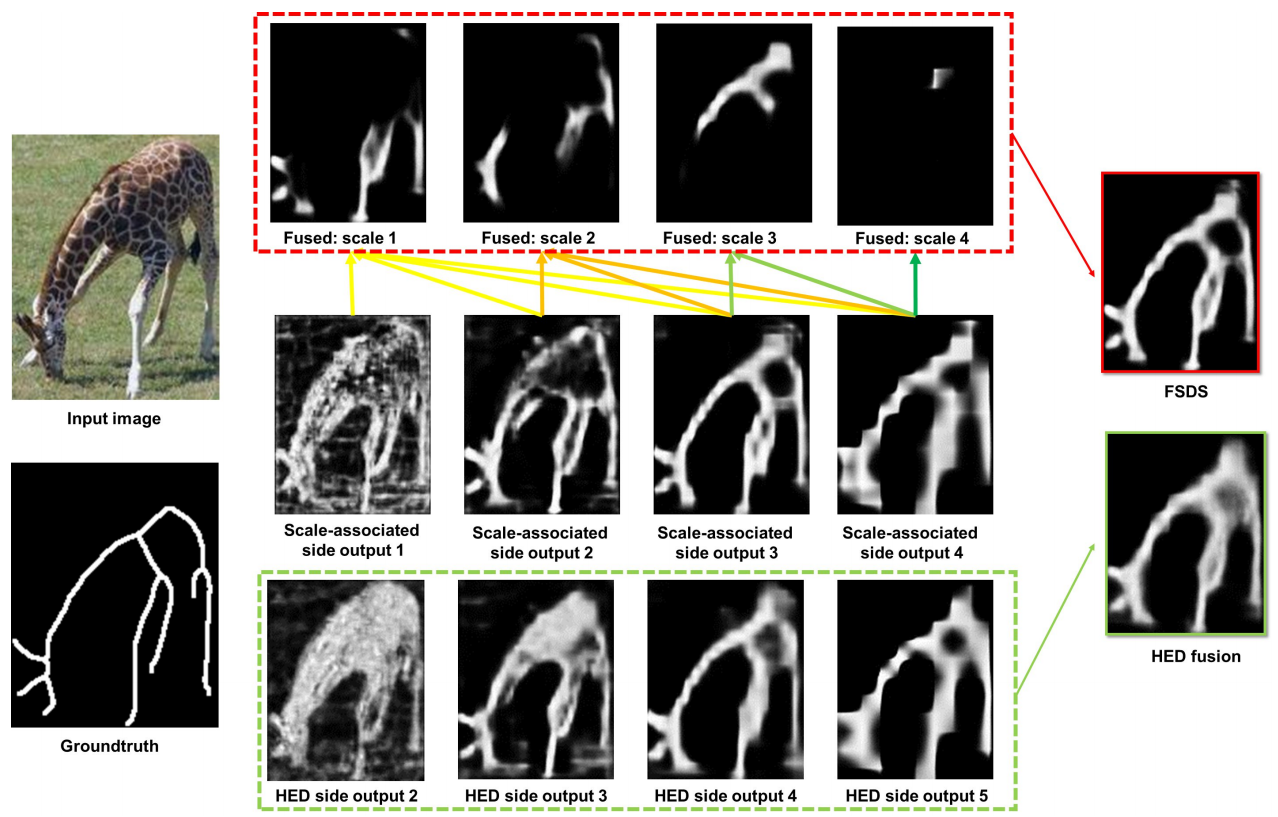
\includegraphics[scale=0.3]{figures/lmsds_hed.png}
\caption{本文所提出模型(FSDS)与HED中间输出结果的对比。FSDS具有区分不同骨架尺度像素点的能力,而HED不具备这种能力。}
\label{fig:fsds_hed}
\end{figure}

\subsection{实验结果和性能分析}
这一节介绍实验细节并将我们所提出的骨架提取算法与其他算法进行性能比较。
\subsubsection{实现细节}
我们的网络模型基于FCN~\cite{long2015fully}和HED~\cite{xie2015holistically}。在训练开始之前整个网络的参数用 VGG16初始化~\cite{Simonyan14c}。

\vspace{1em}
\noindent \textbf{模型参数} 整个模型有以下几个超参数:1)mini-batch(1),2)初始学习率(1e-10),3) momentum(0.9),4)参数$\mathbf{A}$的初始值($\frac{1}{M}$,$M$是SSO个数),5)weight-decay(2e-4),6)训练时的最大迭代次数(20k)。

\vspace{1em}
\noindent \textbf{数据扩增(data augmentation)} 数据扩增是一种重要的产生充足的训练样本和提升模型泛化能力(generalization)的方式。我们用3种角度(90, 180, 270)旋转,沿不同的轴翻转(左右翻转,上下翻转,不翻转),以不同倍率
resize图像( 0.8, 1.0, 1.2 )来扩增训练集。通过以上几种方式的组合,最终数据集的扩增倍率为36。在对图像作以上变换的时候,对应的骨架图ground-truth也要随之变换,尤其值得注意的是,当对图像进行resize放大和缩小的时候,骨架的
尺度也要发生变化。

\subsection{性能比较}
我们比较了本文所提出方法和其它几种主流的骨架检测方法,包括基于图像处理的方法( Lindeberg's method ~\cite{lindeberg1998edge}),基于机器学习和分割连接的方法(Levinshtein's method ~\cite{levinshtein2013multiscale})以及三个
逐像素分类/回归的方法(Distance Regression~\cite{sironi2014multiscale},MIL~\cite{tsogkas2012learning},MISL~\cite{shen2013skeleton})和一个基于深度学习的方法(HED~\cite{xie2015holistically})。上述所有方法我们都使用作者提供
的源代码和默认的参数进行训练和检测。对于同样基于深度学习的方法HED,我们迭代充分直至收敛。检测完成的骨架图经过标准的非极大值抑制算法~\cite{dollar2015fast}进行后处理得到细化后的骨架,最后的性能比较在细化后的骨架上进行。

\subsubsection{评价标准}
不同方法之间使用~\cite{tsogkas2012learning}一样的算法计算,骨架检测的性能由F-measure=\\$\frac{2*\text{Precision}\cdot\text{Recall}}{\text{Precision}+\text{Recall}}$的最大值和pr曲线来衡量。Precision和Recall由检测出的骨架图
和骨架图ground-truth计算得到。

为了得到pr曲线,所检测到的骨架图首先通过一个阈值转换为二值图,然后与 ground-truth 骨架图进行匹配,匹配过程中允许很小的定位误差,也就是说检测出的骨架和ground-truth之间允许存在很小的位置偏移。如果一个检测出的骨架点和至少
一个ground-truth骨架点匹配上,那么这个点就会作为true-positive,如果一个检测出的骨架点匹配不到任何ground-truth骨架点,那么就会作为false-positive。通过使用不同的阈值,我们得到一系列的precision和recall值,然后用这些点得到pr曲线。

\subsubsection{SK-LARGE}
SK-LARGE是我们收集并公开的一个骨架检测的数据集,包含756张训练用图和745张测试用图以及对应的骨架ground-truth。表~\ref{tb:f1_skl}是SK-LARGE上骨架提取算法的F-measure和平均每张图的检测用时。FSDS和LMSDS是本文所提出的方法,
其中FSDS只进行骨架提取,LMSDS是结合了骨架尺度预测的多任务网络。从结果可以看到,不管是传统的图像处理方法,还是基于机器学习的逐像素分类/回归算法均表现不佳,说明骨架提取是一个很难的任务。本文所提出的方法明显优于其他算法,
并且优于同样基于深度学习的HED~\cite{xie2015holistically}。同时,由于GPU的强大运算能力,我们的算法可以以20帧每秒的速度处理图像,达到实时处理的要求,运行时间上相比其它算法也有很大的优势。图~\ref{fig:pr_skl}是不同方法的pr
曲线,图~\ref{fig:examples_skl}是几个骨架检测结果的例子。从结果可以看出,基于骨架提取+尺度预测多任务的方法不仅可以预测到骨架的尺度,对骨架提取本身也有性能提升。
\begin{center}
\begin{tabular}{l*{6}{c}r}
Method            & F-measure & runtime(ms) \\
\hline
Lindeberg~\cite{lindeberg1998edge} & 0.270 & 4.05  \\
Levinshtein~\cite{levinshtein2013multiscale} & 0.243 & 146.21  \\
Lee~\cite{sie2013detecting} & 0.255 & 609.10  \\
MIL~\cite{tsogkas2012learning} & 0.293 & 42.40  \\
MISL~\cite{shen2016multiple} & 0.402 & 0.05  \\
HED~\cite{xie2015holistically} & 0.497 & 0.05 \\
\textbf{FSDS}     & 0.633 &0.05 \\
\textbf{LMSDS}     & 0.649 &0.05 \\
\hline
\end{tabular}
\captionof{table}{SK-LARGE数据集上的F-measure和运行时间。}
\label{tb:f1_skl}
\end{center}
\begin{figure}[H]
\centering
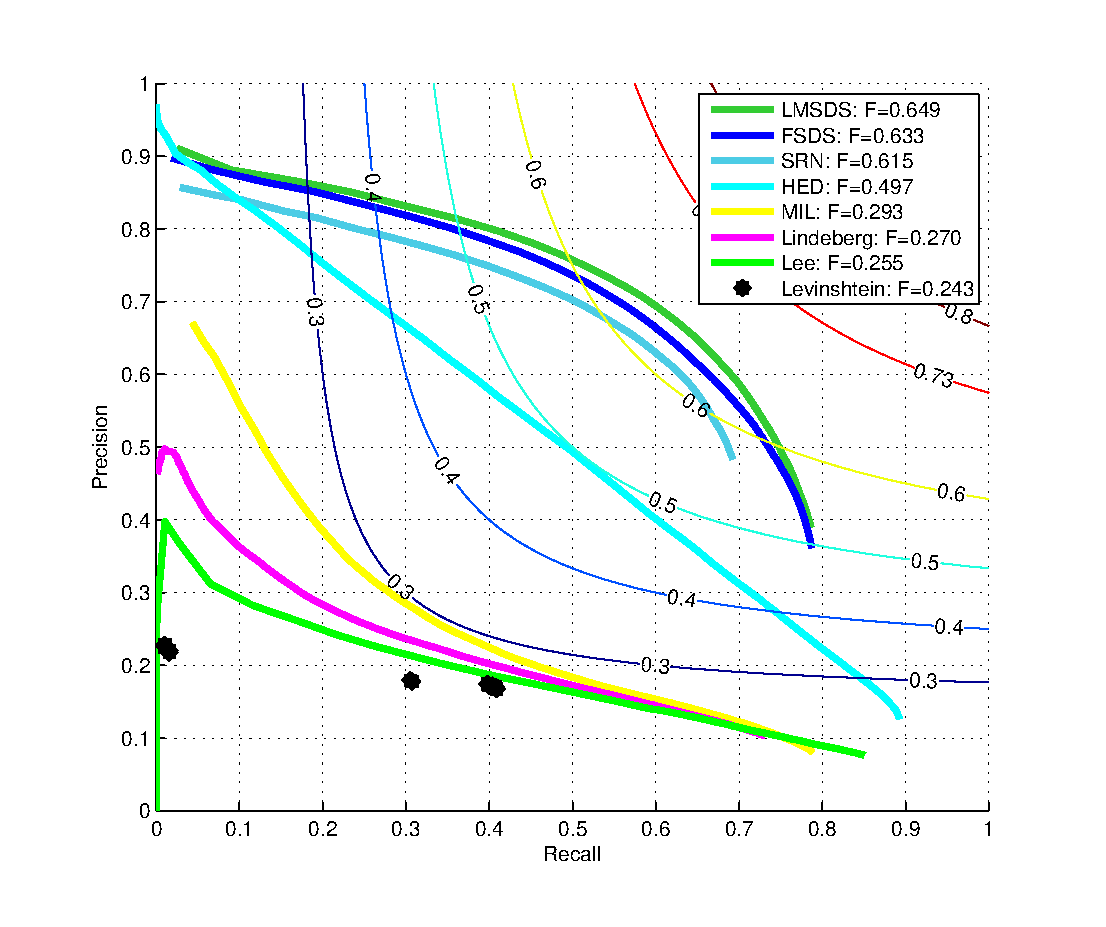
\includegraphics[scale=0.5]{figures/pr-skl.eps}
\caption{SK-LARGE数据集上的骨架提取结果,方法按照best F-measure排序。}
\label{fig:pr_skl}
\end{figure}
\begin{figure}[!htb]
\centering
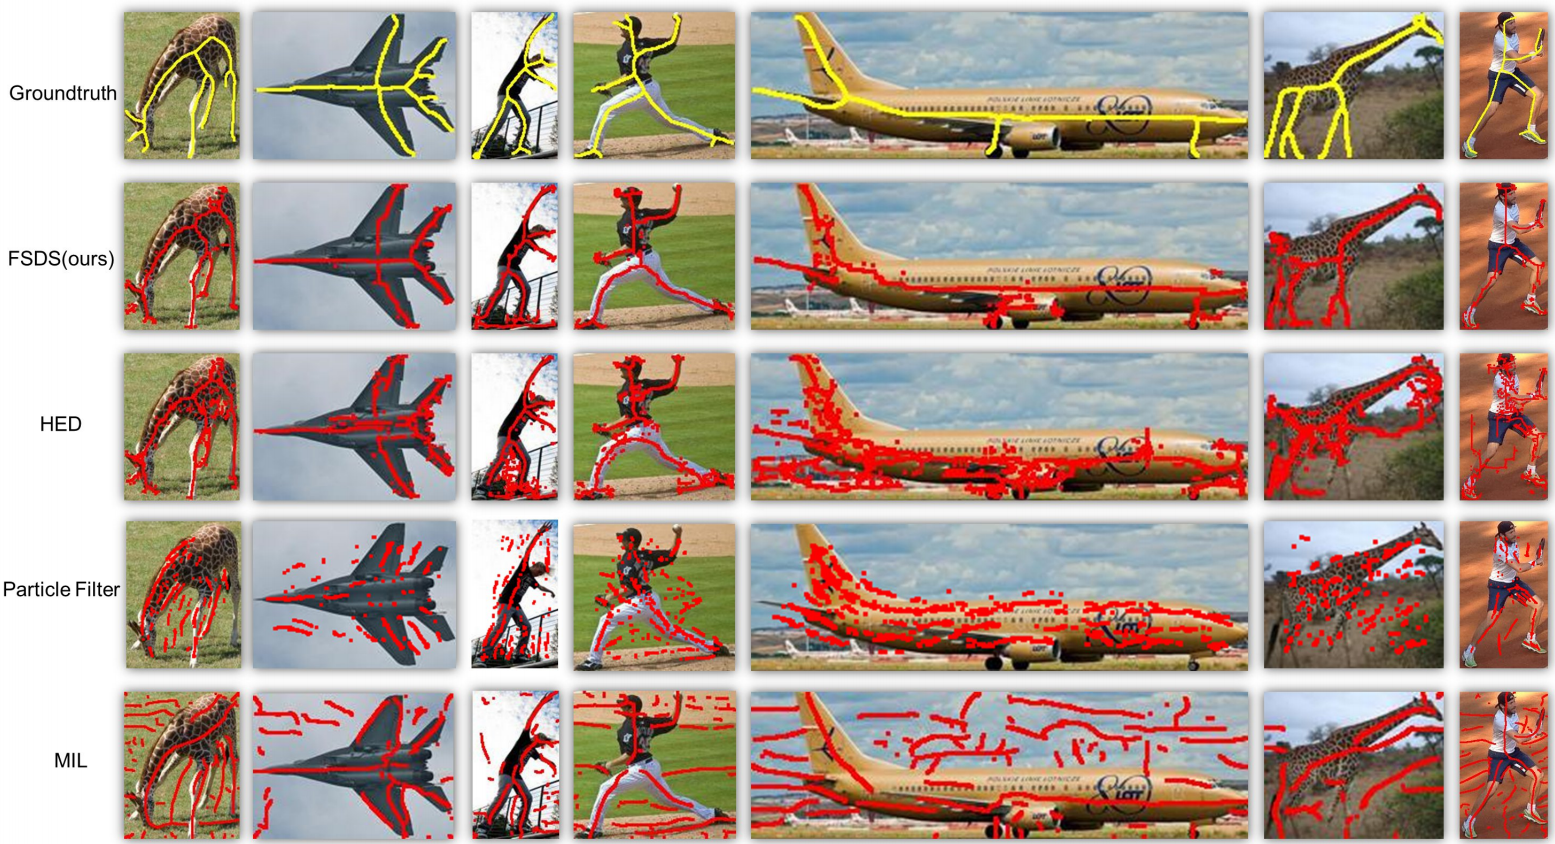
\includegraphics[scale=0.25]{figures/examples_skl.png}
\caption{SK-LARGE数据集上骨架提取的结果,第一排中黄色骨架为ground-truth。}
\label{fig:examples_skl}
\end{figure}


\subsubsection{WH-SYMMETRY}
WH-SYMMAX~\cite{shen2016multiple}数据集包含328张马的图像,其中前228张用于训练,后 100 张用于测试。图~\ref{fig:pr_wh}是WH-HORSE数据集上的pr曲线,图~\ref{fig:examples_wh}是WH-SYMMAX上骨架提取结果的几个例子,
表~\ref{tb:f1_wh}是检测结果的定量比较。
\begin{center}
\begin{tabular}{l*{6}{c}r}
Method            & F-measure & Avg Runtime(Sec) \\
\hline
Lindeberg~\cite{lindeberg1998edge} & 0.277 & 5.75  \\
Levinshtein~\cite{levinshtein2013multiscale} & 0.174 & 105.51  \\
Lee~\cite{sie2013detecting} & 0.223 & 716.18  \\
Particle Filter~\cite{widynski2014local} & 0.334 & 13.9  \\
Distance Regression~\cite{sironi2014multiscale} & 0.103 & 5.78  \\
MIL~\cite{tsogkas2012learning} & 0.365 & 51.19  \\
MISL~\cite{shen2016multiple} & 0.402 & 78.41  \\
HED~\cite{xie2015holistically} & 0.732 & 0.06 \\
\textbf{FSDS}     & 0.769 &0.07 \\
\textbf{LMSDS}     & 0.779 &0.07 \\
\hline
\end{tabular}
\captionof{table}{WH-SYMMETRY数据集上的F-measure值和运行时间。}
\label{tb:f1_wh}
\end{center}
\begin{figure}[H]
\centering
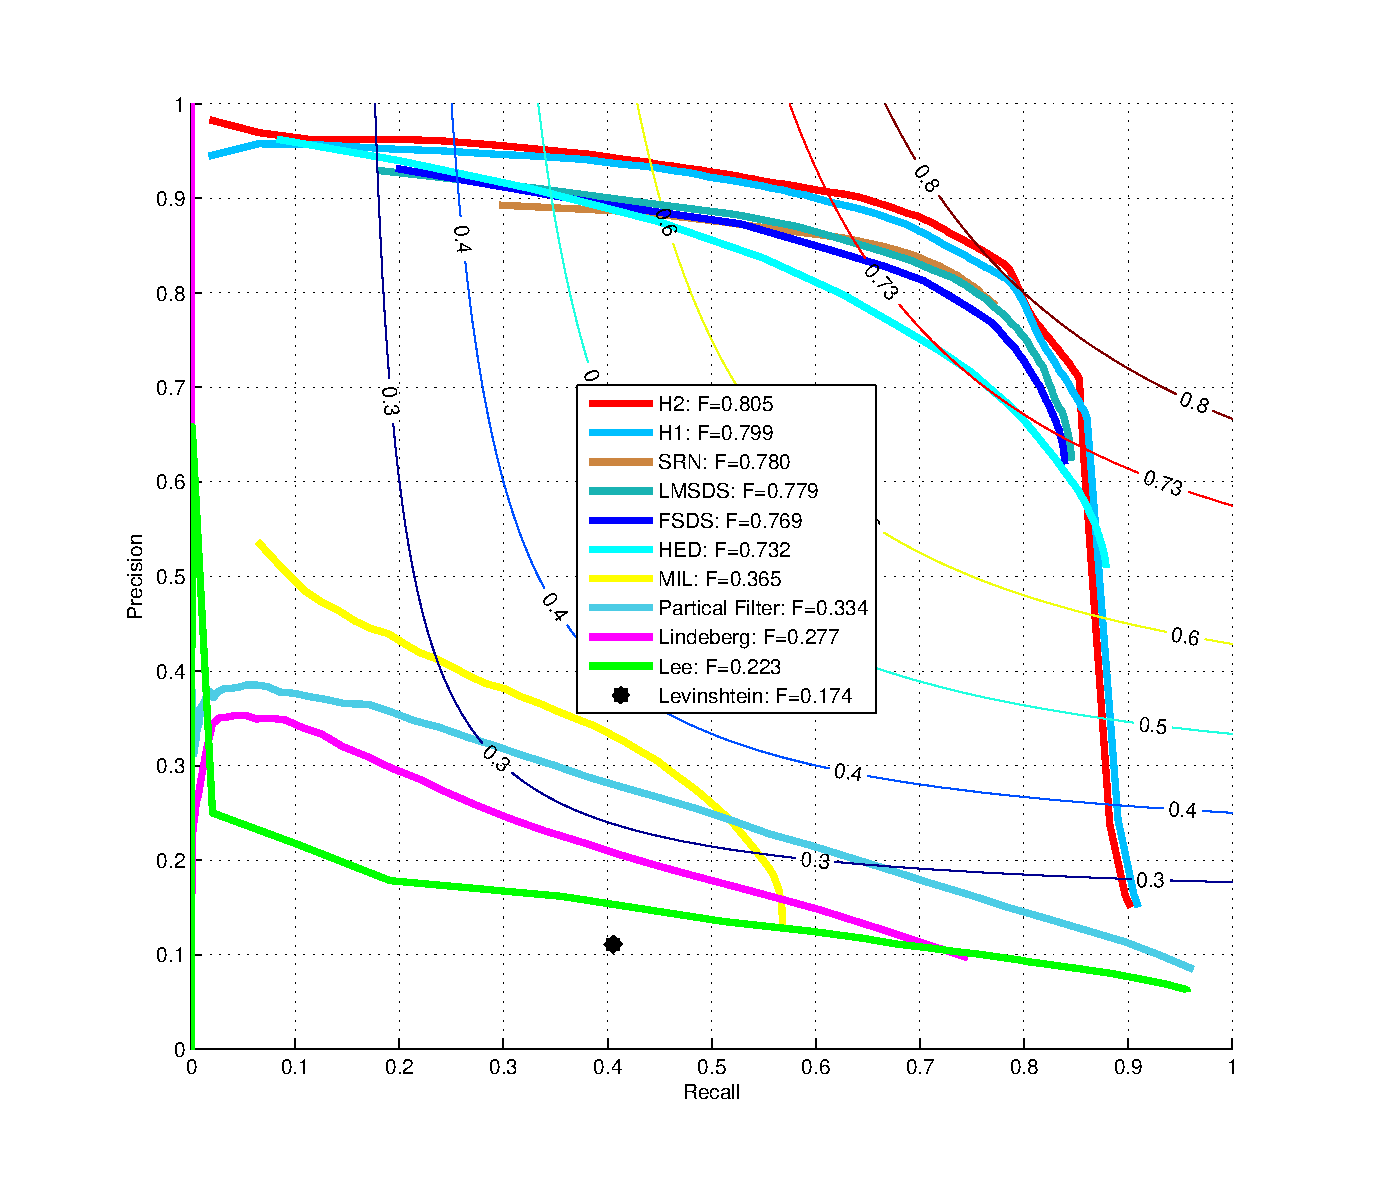
\includegraphics[scale=0.5]{figures/pr-wh}
\caption{WH-SYMMETRY数据集上的骨架提取结果,方法按照best F-measure排序。}
\label{fig:pr_wh}
\end{figure}
\begin{figure}[!htb]
\centering
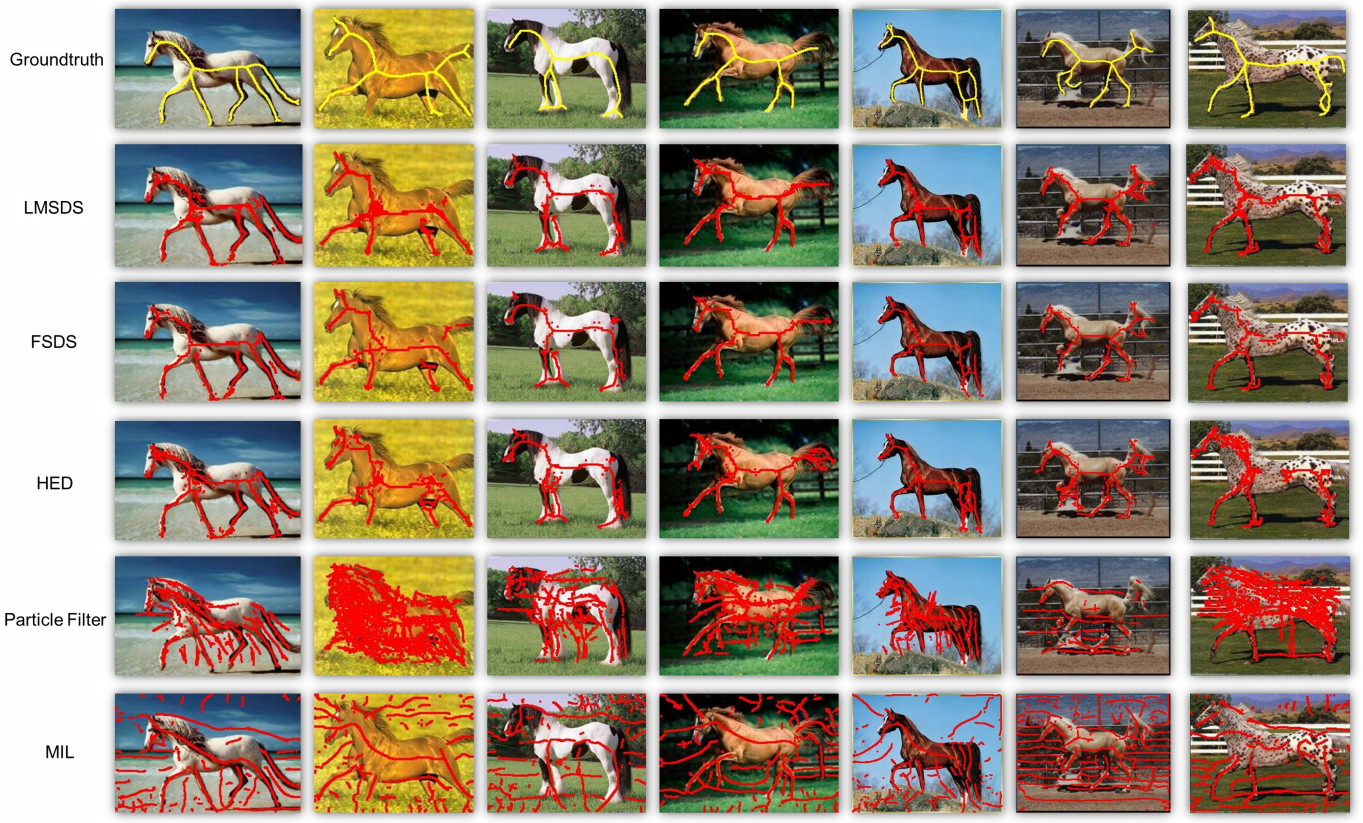
\includegraphics[scale=0.25]{figures/examples_wh.png}
\caption{WH-SYMMETRY数据集上骨架提取的结果,第一排中黄色骨架为ground-truth。}
\label{fig:examples_wh}
\end{figure}

\subsubsection{跨数据集的交叉验证}
为了进一步验证所提出模型的泛化能力(generalization),我们进行了两个数据集的交叉验证(在A数据集上训练并在B数据集上测试)。交叉验证结果表明,本文所提出方法相比于其他基于机器学习的方法具有更好的泛化能力,
表~\ref{tb:cross_val}是交叉验证的定量结果。
\begin{center}
\begin{tabular}{l*{6}{c}r}
Method            & Train/Test & F-measure \\
\hline
MIL~\cite{tsogkas2012learning} & SK-LARGE/WH-SYMMAX & 0.350 \\
HED~\cite{xie2015holistically} & SK-LARGE/WH-SYMMAX & 0.583 \\
\textbf{LMSDS}                 & SK-LARGE/WH-SYMMAX & 0.701 \\
\hline
MIL~\cite{tsogkas2012learning} & WH-SYMMAX/SK-LARGE & 0.357 \\
HED~\cite{xie2015holistically} & WH-SYMMAX/SK-LARGE & 0.420 \\
\textbf{LMSDS}                 & WH-SYMMAX/SK-LARGE & 0.474 \\
\hline
\end{tabular}
\captionof{table}{WH-SYMMAX和SK-LARGE数据集上交叉验证的结果。}
\label{tb:cross_val}
\end{center}
\subsection{本章小结}
本章提出了一种基于尺度相关的边输出(SSO:scale-associated side-output)的骨架提取算法,利用感受野不同的边输出解决骨架提取中的尺度未知问题,对图像背景和物体上的噪声不敏感。在SK-LARGE和WH-SYMMAX数据集上的实验结果表明
本章所提出的算法得到的骨架明显优于其他主流方法,同时本章所提出的骨架提取算法能够准确预测骨架的尺度,骨架尺度作为骨架的一个补充,有更多的应用价值,相关内容将在后续章节介绍。本章研究内容已发表在计算机视觉领域
国际顶级会议IEEE Conference on Computer Vision and Pattern Recognition, 2016。

%%%%%%%%%%%%%%%%%%%%%%%%%%%%%%%%%%%%%%%%%%%%%%%%%%%%%%%%%%%%%%%%%%%%%%%%%%%%%%%%%%%
%%%%%%%%%%%%%%%%%%%%%%%%%%%%%%%%%%%%%%%%%%%%%%%%%%%%%%%%%%%%%%%%%%%%%%%%%%%%%%%%%%%
\pagebreak
\section{骨架在物体识别与检测中的应用}%\label{sec:seg_recover}
本章介绍骨架在物体识别中的应用,包含三个方面:1)利用检测到的骨架恢复物体分割,2)利用骨架为目标检测提取候选窗口,3)利用所提出的骨架检测算法检测对称物体(航拍图中的道路和自然图像中的文本行)。由于骨架包含了物体各部件的连接信息,而骨架尺度补充了物体的形状信息,通过骨架和骨架尺度我们就能恢复出
物体的形状;同时骨架位于图像前景区域,通过检测到的骨架可以抑制位于背景上的候选窗口,为目标检测算法提供更优质的候选窗口。图像中有些目标和骨架一样具有对称性,因此本文所提出的骨架检测算法同样适用于这些对称物体的检测。

\subsection{利用骨架和骨架尺度恢复物体分割}\label{sec:seg_recover}
本节介绍骨架检测的第一个应用,即利用骨架和骨架尺度,通过作以骨架点为中心,骨架尺度为半径的圆得到物体的分割。由于所检测骨架并没有区分物体的类别,理论上所有物体都将被分割出来,因此得到的分割可以认为是图像的\textbf{前景分割}。
\begin{figure}[!htb]
\centering
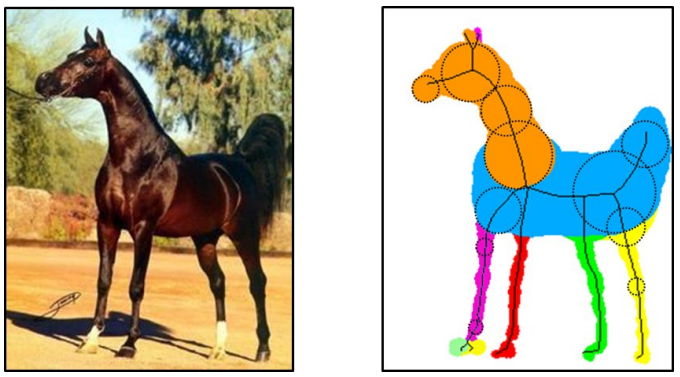
\includegraphics[scale=0.3]{figures/sk2seg.png}
\caption{从骨架到分割。}
\label{fig:sk2seg}
\end{figure}
上述从骨架得到物体分割的过程可以公式化为:
\begin{equation}
\text{seg}_i =
\begin{cases}
 1 \ \text{if distance(}x_i,\text{sk}_i\text{)}<\hat{s}_i \\
0 \ \text{others}
\end{cases}
\label{eq:sk2seg}
\end{equation}
式~\ref{eq:sk2seg}中$\text{distance(}\cdot,\cdot \text{)}$为图像中两像素之间的距离,$\text{sk}_i$是\textbf{离像素点$x_i$最近的骨架点},$\hat{s}_i$是预测的$x_i$点的骨架尺度,$\text{seg}_i$是得到的分割图像素点$i$的值,
最后得到的分割图 seg 是一个二值图(binary map)。

\subsubsection{使用量化骨架尺度恢复物体分割}
如第3章所述,本文所提出的骨架检测方法实际上是得到了像素点$x_j$属于每一个量化骨架类别$k$的概率$f_{jk},(\sum_{k=0}^K f_{jk})=1$,$f_{jk}$是式~\ref{eq:fuse_loss}中多个SSO融合之后的预测。根据式~\ref{eq:get_sk},最后的骨架
实际上是多种量化类别概率的和:$P(x_j\text{is skeleton})=\sum_{k=1}^K f_{jk}=1-f_{j0}$。因此得到骨架检测的融合输出$f_{jk}$,实际上已经获取了关于骨架点尺寸的一个粗略估计。

利用$f_{jk}$我们可以粗略的估计骨架的尺寸$\hat{s}_j = r_{*i}$,式中$*i$根据式~\ref{eq:most_likely_cls}得到,$r_i$为第$i$个SSO的感受野(receptive field)。也就是说我们先预测出像素点$x_j$的量化骨架类别,然后用该类别对应
SSO的感受野作为$x_j$的骨架尺度,最后使用式~\ref{eq:sk2seg}的方法得到物体分割。本文所用网络4个SSO的感受野分别是$(14,40,96,192)$,因此如果像素点$x_j$的真实尺度是$s_j = 15$,那么估计出来的尺度就是第二个SSO的感受野,
也就是40,如果$s_j = 41$,那么估计出来的尺度$\hat{s}_j = 96$,这样得到的尺度显然是十分粗糙的,而且\textbf{骨架真实尺度越大,估计出的误差越大}。
\begin{figure}[!htb]
\centering
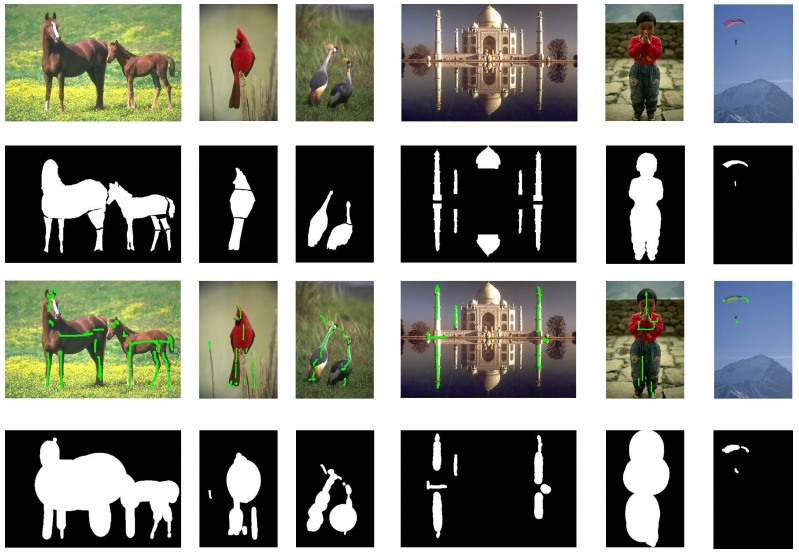
\includegraphics[scale=0.3]{figures/seg_fsds.png}
\caption{利用量化骨架尺度恢复物体分割的结果。}
\label{fig:seg_fsds}
\end{figure}
图~\ref{fig:seg_fsds}是利用量化骨架尺度恢复物体分割的部分实验结果,可以看出恢复的结果比较粗糙,特别是对于骨架尺度较大的点(图中马的身子),分割结果不理想。值得注意的是,图中第四列建筑物的分割没有恢复出来,并不是骨架尺度估计的不准,
而是其骨架尺度已经超出了所有 SSO 感受野(最大为192),无法检测其骨架。

\subsubsection{使用ScalePred-SSO准确预测骨架尺度}
通过量化骨架尺度估计出的骨架尺度误差较大,得到的分割会不准确,特别是在物体骨架尺度比较大的地方。比如图~\ref{fig:seg_fsds}中马的身体部位就显得很胖,这是身体部分的骨架尺度估计不准造成的。

为了得到与物体更匹配的分割结果,我们必须更精确地估计骨架尺度,因此在多输出网络的基础上我们拓展出多任务网络,同时检测骨架并估计骨架尺度。根据式~\ref{eq:most_likely_cls}我们可以得到某个像素点最有可能属于的量化尺度类别$i*$,
然后根据式~\ref{eq:get_sk_scale},使用第$i*$个ScalePred-SSO预测的骨架尺度值作为式~\ref{eq:sk2seg}中的$\hat{s}_i$进行前景分割。

\subsubsection{实验结果与分析}
我们在SK-LARGE和WH-SYMMAX两个数据集上进行了图像前景分割的实验,然后分别根据MS-COCO~\cite{chen2015microsoft}和Weizmann Horse~\cite{borenstein2002class}提供的分割ground-truth标注来评价不同算法的性能。我们对比了多个当前主流的
图像分割算法,其中CPMC~\cite{carreira2010constrained}和 Shape Sharing~\cite{kim2012shape}都是基于图分割(graph cut)的无监督方法,每幅输入图像都产生大量互有重叠的分割片段(segmentation mask),我们取其中与ground-truth最匹配的
一个作为分割结果;FCN~\cite{long2015fully}是一种语义分割的方法,在第二章已经介绍,我们取前景物体对应类别的分割片段作为分割结果。

图~\ref{fig:seg_wh}是WH-SYMMAX数据集上不同算法得到的分割结果。可以看到,FCN-8s对于马身上花纹很敏感,FSDS(使用量化骨架尺度)得到的分割图马普遍比较“胖”,这是由于尺度预测不准造成的,而LMSDS能得到更为精确的分割结果,这归功于
多任务网络对骨架和骨架尺度的准确预测。
\begin{figure}[H]
\centering
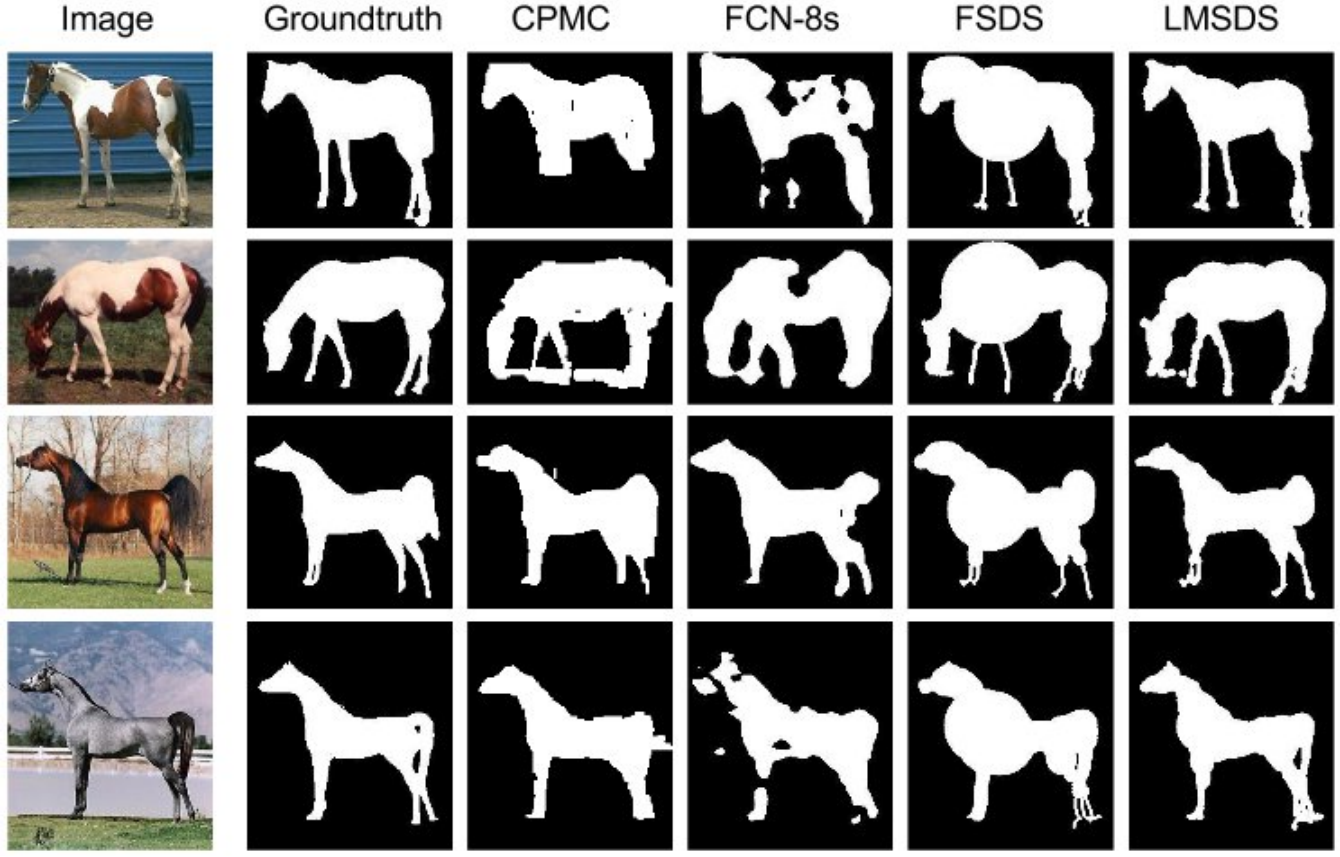
\includegraphics[scale=0.3]{figures/seg_wh.png}
\caption{WH-SYMMAX数据集上不同算法得到的分割结果。}
\label{fig:seg_wh}
\end{figure}
图~\ref{fig:seg_skl}是SK-LARGE数据集上的分割结果。与WH-SYMMAX上的结果类似, FSDS 对骨架尺度估计不准,导致物体普遍偏“胖”,LMSDS能得到不错的分割结果。
\begin{figure}[H]
\centering
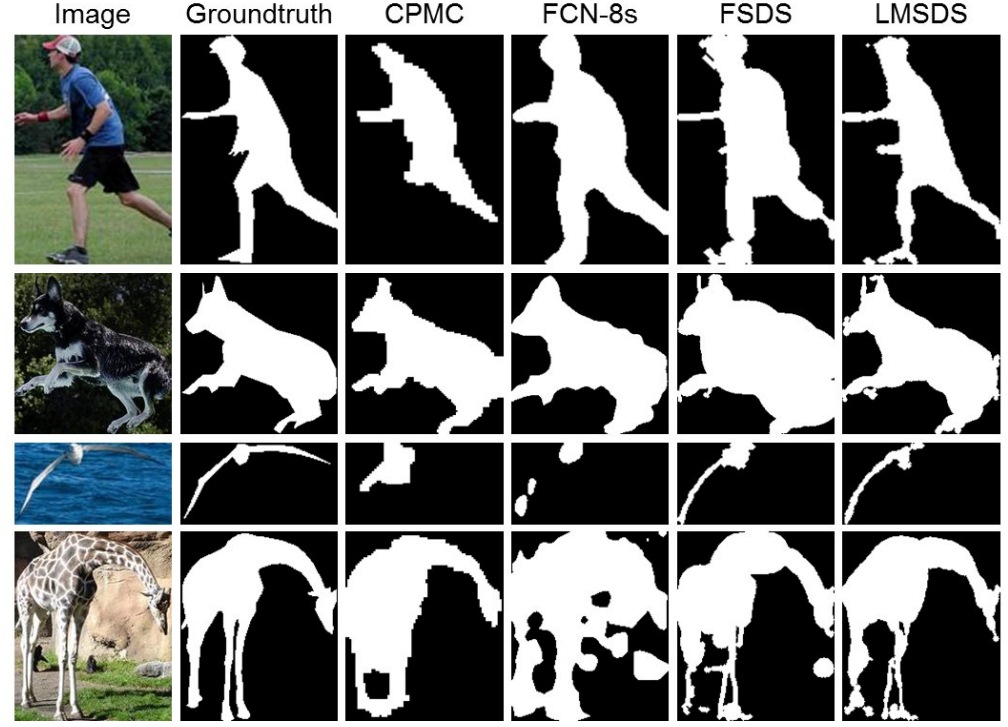
\includegraphics[scale=0.3]{figures/seg_skl.png}
\caption{SK-LARGE数据集上不同算法得到的分割结果。}
\label{fig:seg_skl}
\end{figure}

同时为了全面地比较不同算法的性能,我们采用了~\cite{demirci2006object}一样的评价标准,让分割结果的每一个像素有一个置信度,对每一个分割的前景点$j$,我们取距离其最近的骨架点的响应作为其置信度$\text{seg}^{'}_j$,即
\begin{equation}
\text{seg}^{'}_j = \text{seg}_j * \hat{y}_i
\label{eq:soft_seg}
\end{equation}
其中$\text{seg}$在式~\ref{eq:sk2seg}中定义,$\hat{y}_i$是式~\ref{eq:get_sk}得到的骨架响应,$i$是距离$j$最近的骨架点。与骨架检测结果的评价类似,我们可以使用不同的阈值作用在$\text{seg}^{'}$上得到不同的二值分割结果,每个分割
都能得到一个准确率(precision)和召回率(recall),然后计算各自的F-measure=$\frac{2*\text{Precision}\cdot\text{Recall}}{\text{Precision}+\text{Recall}}$,最后在整个数据集上取F-measure的最大值。
同时我们也计算了由式~\ref{eq:sk2seg}得到的
“硬”分割结果和ground-truth的覆盖率(Covering)。假设我们有人工标注的$\text{gt}$和检测出的结果$\text{det}$,它们都由若干个分割片段$\text{gt}_i, \text{det}_i$组成,覆盖率按照以下公式计算:
\begin{equation}
\text{Covering(det, gt)} = \sum_{i=1}^M \frac{\text{gt}_i \cap \text{det}_i}{\text{gt}_i \cup \text{det}_i} \times  \frac{|\text{gt}_i|}{\sum_j |\text{gt}_j|}
\label{eq:cov}
\end{equation}
式~\ref{eq:cov}中$M$是gt中的分割片段个数,$\text{gt}_i$表示第$i$个ground-truth片段,$\text{det}_i$表示\textbf{与$\text{gt}_i$最匹配的检测片段},$|\cdot|$表示分割片段$\cdot$内的像素点个数。
覆盖率通过计算每个ground-truth片段与和它最匹配的分割片段之间的重合率,并使用ground-truth片段的大小作为权重加权。

表~\ref{tb:seg_eval_wh}是WH-SYMMAX数据集上分割结果的定量比较,其中 “Avg num segments” 表示每张图分割算法所产生的平均分割片段个数,理想的分割检测结果应该是产生尽可能少的分割片段个数的同时达到更高的覆盖率或F-measure。
\begin{center}
\begin{tabular}{l*{6}{c}r}
\hline
Method            & F-measure & Covering(\%) & Avg num segments \\
\hline
Lee~\cite{sie2013detecting} & 0.597 & 43.4 & 253.0   \\
MIL~\cite{tsogkas2012learning} & 0.278 & 30.7 & 8.2  \\
Shape Sharing~\cite{kim2012shape} & 0.857 & 75.4 & 879.8 \\
CPMC~\cite{carreira2010constrained} & 0.872 & 80.1 & 511.2 \\
FCN-8s~\cite{long2015fully} & 0.823 & 72.1 & 2.3 \\
\textbf{FSDS}(ours)     & 0.838 & 72.5 & 1.7 \\
\textbf{LMSDS}(ours)    & 0.902 & 82.4 & 1.3 \\
\hline
\end{tabular}
\captionof{table}{WH-SYMMAX数据集上的分割结果定量比较。}
\label{tb:seg_eval_wh}
\end{center}
  
如前文所述,CPMC算法会产生大量的分割片段(segments),例如在 WH-SYM\\MAX 数据集上平均每张图产生了511个,我们取其中与ground-truth最匹配的片段作为分割结果。由于检测到的骨架并不一定是连续的,因此
本文所提出的方法( FSDS 和 LMSDS )也会在一张图上产生多个分割片段,例如FSDS算法在WH-SYMMAX数据集上平均每张图产生1.7个分割片段。从分割质量上来讲,我们希望一个算法能够产生尽可能少的分割片段并取得
比较高的覆盖率和F-measure。从WH-SYMMAX数据集上的定量比较结果上来看,无论是FSDS还是LMSDS都能产生比基于深度学习的算法FCN-8s更好的分割结果,同时产生最的分割片段数目。而 CPMC 和 Shape Sharing虽然
能够得到比较好的分割结果,但是它产生了数量巨大的分割片段,并且并不知道其中每一个片段的具体语义。

表~\ref{tb:seg_eval_skl}是SK-LARGE数据集上分割结果。SK-LARGE数据集中的图像有更复杂的背景和更多的物体类别,会影响到骨架检测的质量,因此相比在WH-SYMMAX数据集上,SK-LARGE数据集上FSDS和LMSDS两种
方法会产生更多的分割片段。方法会产生更多的分割片段。
\begin{center}
\begin{tabular}{l*{6}{c}r}
\hline
Method            & F-measure & Covering(\%) & Avg num segments \\
\hline
Lee~\cite{sie2013detecting}         & 0.496 & 33.8 & 210.5 \\
MIL~\cite{tsogkas2012learning}      & 0.268 & 27.5 & 8.4   \\
Shape Sharing~\cite{kim2012shape}   & 0.854 & 75.4 & 716.2 \\
CPMC~\cite{carreira2010constrained} & 0.896 & 81.8 & 287.0 \\
FCN-8s~\cite{long2015fully}         & 0.840 & 74.2 & 3.8   \\
\textbf{FSDS}(ours)                 & 0.814 & 69.1 & 2.0   \\
\textbf{LMSDS}(ours)                & 0.873 & 78.1 & 2.1   \\
\hline
\end{tabular}
\captionof{table}{SK-LARGE数据集上的分割结果定量比较。}
\label{tb:seg_eval_skl}
\end{center}

\subsection{利用骨架提取目标检测候选窗口}
本节介绍骨架的另一个应用:为目标检测提取候选窗口。候选窗口检测算法( object proposal detection )有时候也称为似物性检测(objectness detection),是一种为目标检测提供高召回率的候选窗口的算法。
目标检测中由于目标位置、大小,形状未知,因此往往依靠用不同比例和大小的滑动窗口遍历图像,并在每一个窗口中进行检测,这种方法的时效性非常差,无法满足实时检测的要求。候选窗口提取算法旨在于为
目标检测提供少量但能够包含图像中所有物体的候选窗口,增强目标检测系统的时效性。这就要求候选窗口检测算法必须:1)提供尽可能少的窗口;2)覆盖尽可能多的物体,因为在候选窗口检测阶段丢失的物体将
永远无法被检测到。由于一个显而易见的事实:物体往往出现在图像前景,或者能检测出物体骨架的区域。因此可以利用骨架检测的结果去提升候选窗口提取算法的性能。

\subsubsection{候选窗口检测算法}
一般而言候选窗口检测有这样一个过程:1)生成一系列的候选窗口,2)为每个窗口赋上“似物性得分(objectness score,以下简称score)”,表示这个窗口中含有物体的可能性,3)输出所有窗口和对应score。一般评价
一个候选窗口检测算法的优劣我们会采用固定窗口个数的情况下比较检测率(Recall),实际上这跟我们对候选窗口检测的期望是一致的:用尽可能少的窗口,包含图像中尽可能多的物体。
对于一个检测窗口,我们根据IoU(intersection over union)判断是否true-positive。IoU=$\frac{\text{det}\cap \text{gt}}{\text{det}\cup \text{gt}}$,det为检测到的窗口,gt为 ground-truth 窗口,
IoU为检测窗口与 ground-truth 窗口的交集除以他们的并集,体现了检测窗口与 ground-truth 窗口的匹配程度。

例如,我们可以规定IoU$>$0.6的窗口为true-positive,只有IoU$>$0.6的窗口才会被认为成功检测到物体,那么我们可以画出一条检测窗口个数与检测率( Recall )的曲线来表现候选窗口提取算法的性能。

Edge Boxes~\cite{zitnick2014edge}利用了“物体往往由闭合轮廓包围”这一事实,通过计算候选窗口中所检测出轮廓的得分来确定。

\subsubsection{使用骨架和分割改善Edge Boxes}
Edge Boxes~\cite{zitnick2014edge}是一种利用"物体被闭合轮廓包围"这一假设检测候选窗口的算法。首先Edge Boxes初始化大量的候选窗口(bounding box,以下简称bbox),然后用~\cite{dollar2015fast}提取
输入图像的轮廓,然后通过设定一系列的规则对bbox内部的轮廓片段进行评分,并将bbox内所有轮廓片段的得分求和作为该bbox的score。该方法假设合理而且计算简单,检测结果也不错。

由于图像背景和物体内部的纹理变化会对轮廓检测带来干扰,而且“物体由闭合轮廓所包围”这一假设本身在一些情况下不成立,导致Edge Boxes检测出的bbox也会有一些误检测窗口,例如很多位于背景上的窗口被
赋予很高的似物性得分。基于前文的假设:似物性很高的区域也就是图像中目标物体存在的区域,一定能检测出物体骨架。因此可以使用检测到的骨架和恢复出的分割修正Edge Boxes中窗口的score,提升Edge Boxes窗口检测算法的性能。

假设$h_B^E$是Edge Boxes给窗口$B$的似物性得分,本文通过下式得到窗口$B$新的似物性得分:
\begin{equation}
h_B = \frac{\cup_{\forall \mathcal{M}\cap B \neq \emptyset}(B_{\mathcal{M}}\cap B)}{(\cup_{\forall \mathcal{M}\neq\emptyset}B_{\mathcal{M}})\cup B} \cdot H_B^E
\label{eq:bbox_score}
\end{equation}
式\ref{eq:bbox_score}中$\mathcal{M}$是第\ref{sec:seg_recover}节中恢复出的分割图中的一个分割片段,$B_{\mathcal{M}}$是正好包围$\mathcal{M}$的一个长方形bbox。当一个bbox内所包含分割片段占
该分割片段的比例较小时,说明该bbox并没有完全包围这个物体,
那么这个bbox的score就会被抑制;当窗口内不含分割片段时,说明窗口位于图像背景上,该窗口得分为0。
式\ref{eq:bbox_score}中的评分策略基本上可以抑制位于背景上的干扰窗口的score,从而提升候选窗口检测算法的性能。

\subsubsection{实验结果与分析}
我们在ETHZ Shape Clseese~\cite{ferrari2006object}数据集上测试候选窗口检测算法的性能。将检测到的候选窗口按似物性得分从高到低排序,然后取前N
个窗口计算检测率( detection rate ),只有与物体真实窗口的IoU大于0.6的候选窗口才被认为true-positive。通过取不同的N我们会得到一系列的检测率,最后得到“窗口个数vs检测率”的曲线。
图~\ref{fig:bbox_eval}(a)是 Edge Boxes 和增加了骨架信息的候选窗口提取算法的曲线图。
可以明显看到在不同的窗口个数下增加了骨架信息的两种方法都比Edge Boxes检测率高,特别是当检测窗口比较少的时候优势突出。

图~\ref{fig:bbox_eval}(b)同时对比不同方法产生的似物性得分最高的窗口,红色为Edge Box产生的最似物窗口,绿色是用多尺度相关边输出网络产生的骨架修正了 Edge Boxes 之后的最似物窗口,
蓝色是使用多任务多尺度相关变输出网络修正了Edge Boxes之后的最似物窗口。从实验结果可以明显看出,增加骨架信息会提升Edge Boxes所检测窗口的准确度。例如~\ref{fig:bbox_eval}(b)下排第一个,
Edge Boxes产生的最似物窗口(红色)处于图像背景上,使用骨架修正后可以完全抑制掉这个窗口,输出正确的最似物窗口。

\begin{figure}[H]
\centering
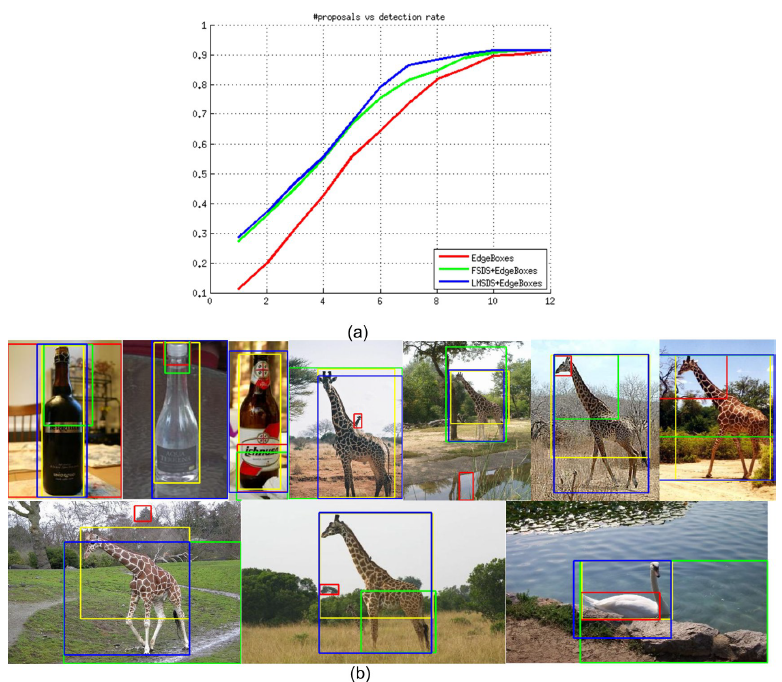
\includegraphics[scale=0.4]{figures/bbox_eval.png}
\caption{在ETHZ Shape Classes~\cite{ferrari2006object}数据集上三种窗口提取算法的性能比较:(a)检测率vs候选窗个数曲线;(b)检测结果样例,黄色窗口为ground-truth,红色窗口为Edge Boxes算法产生的似物得分最高的窗口,
绿色和蓝色窗口分别为Edge Boxes+FSDS和
Edge Boxes+LMSDS产生的最似物窗口。从结果可以明显看出Edge Boxes+LMSDS产生的窗口定位更准确。}
\label{fig:bbox_eval}
\end{figure}

\subsection{基于对称性的图像中目标检测}
对称性是许多图像中目标所具有的一种共同属性,因此本文所提出的骨架检测算法可以用来得到这些具有对称性的目标的对称轴,从而实现对它们的检测。 \\

\noindent \textbf{a)道路检测}

利用计算机自动检测航拍图中的道路在地理信息处理中非常有用,我们可以用本文所提出的骨架检测算法得到航拍图中道路的中轴线,从而定位道路。我们在一个有关航拍道路网络图的数据集~\cite{sironi2014multiscale}上测试并比较了本文所提出的骨架检测算法和文献~\cite{sironi2014multiscale}中所使用的方法。图~\ref{fig:road}是检测结果的定性比较,我们采用与~\cite{sironi2014multiscale}一样的方法将数据集划分为训练集和测试集,同时和骨架检测相同,我们使用pr曲线衡量不同检测算法的性能。图~\ref{fig:road_pr}是两种算法检测结果的pr曲线。实验结果表明本文所提出算法性能优于~\cite{sironi2014multiscale}。
\begin{figure}[H]
\centering
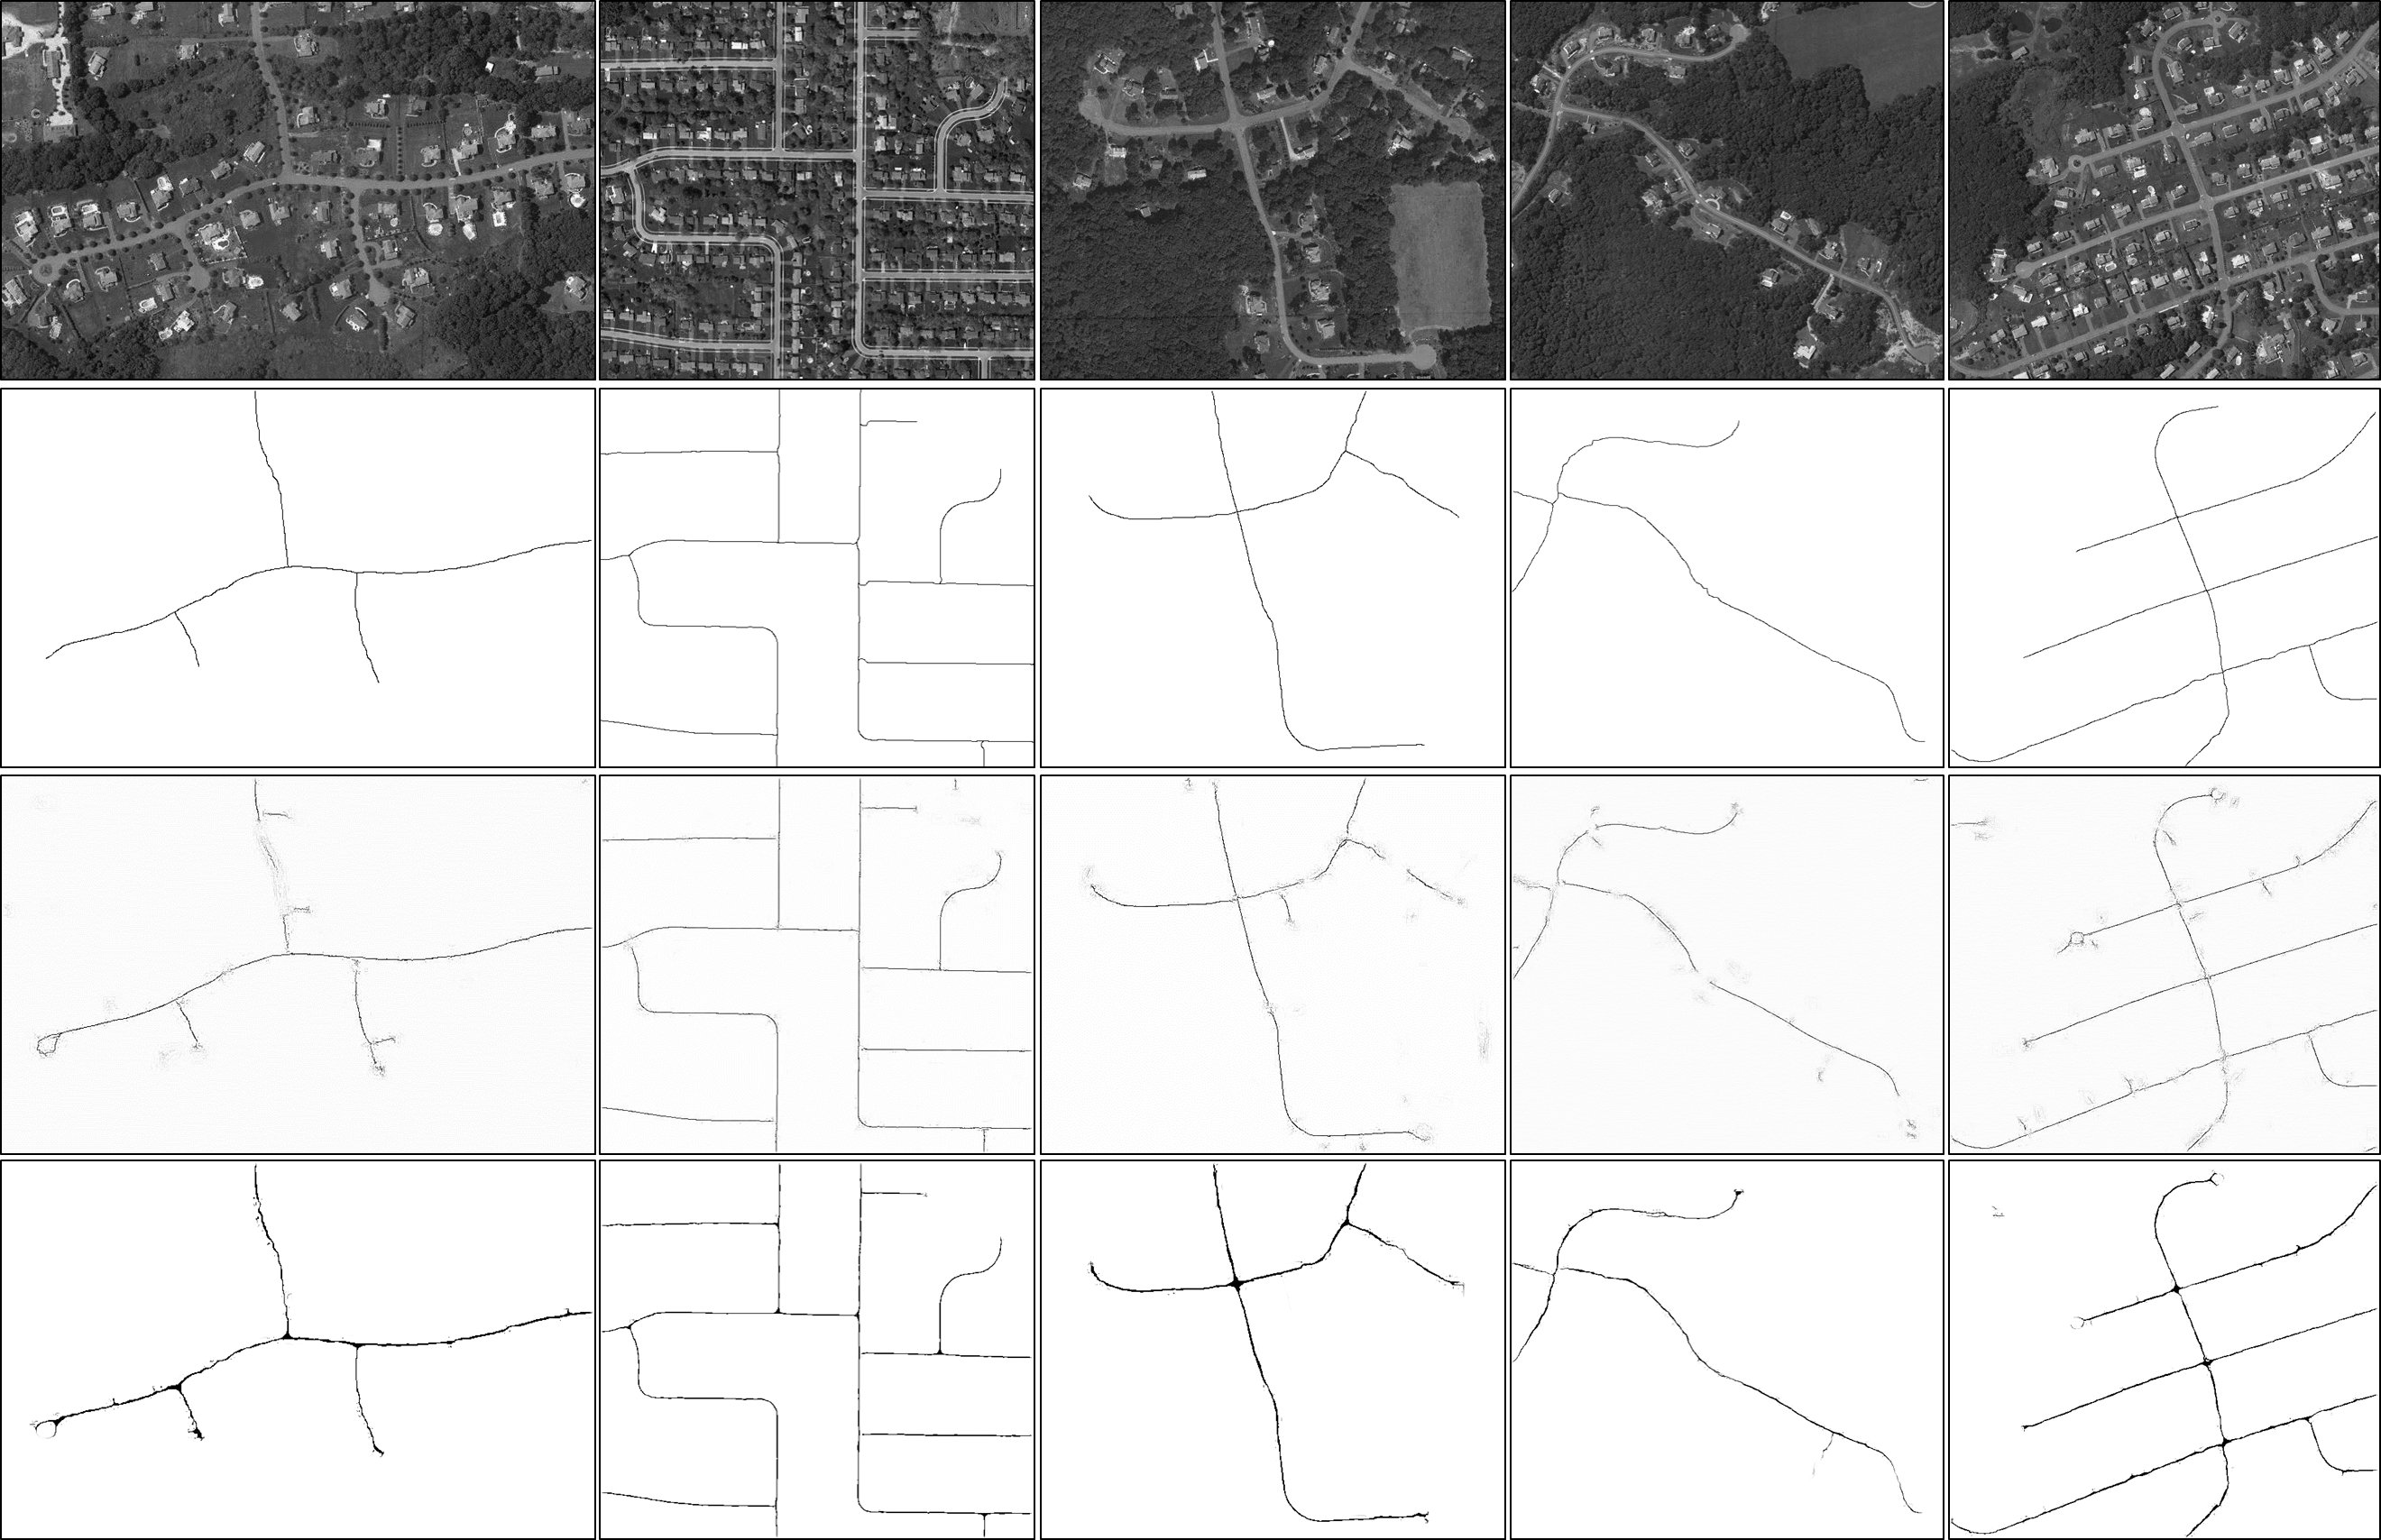
\includegraphics[scale=0.3]{figures/road_detection}
\caption{道路检测的结果,从上到下:第一排,原图;第二排,ground-truth;第三排,~\cite{sironi2014multiscale}的检测结果;第四排,本文所提出算法的结果。}
\label{fig:road}
\end{figure}

\begin{figure}[H]
\centering
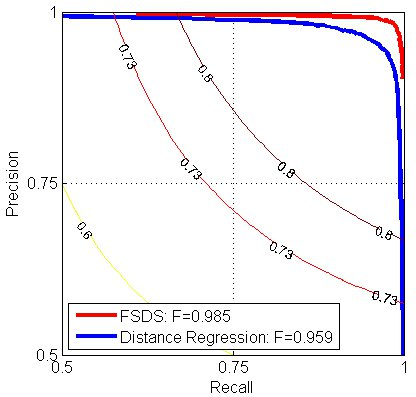
\includegraphics[scale=1]{figures/road_detection_pr}
\caption{道路检测的pr曲线,红色为本文所提出算法,蓝色为~\cite{sironi2014multiscale}。}
\label{fig:road_pr}
\end{figure}

\noindent \textbf{b)文本行检测}

文献~\cite{Zhang15}指出,由于文本和文本周围的背景,自然图像中的文本行通常具有对称性(图~\ref{fig:text_line})。因此我们可以将骨架检测算法应用到文本行检测中来,为文字检测提供候选区域。基于以上思路,我们使用本文所提出的FSDS算法替换~\cite{Zhang15}中的对称性检测算法,在训练阶段,使用文本行的中轴线作为ground-truth来训练对称性检测模型。
\begin{figure}[H]
\centering
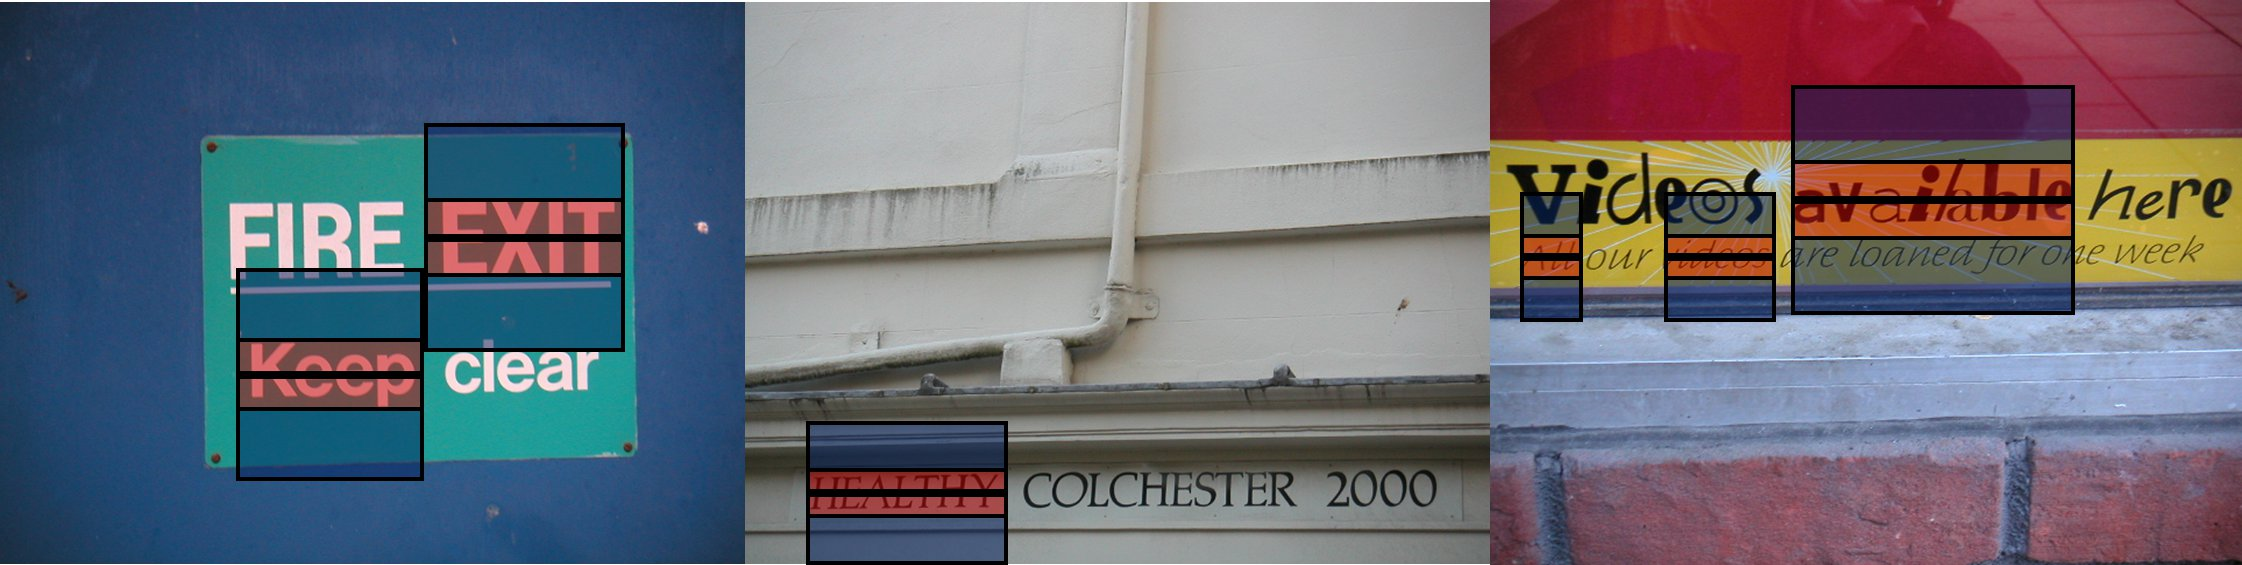
\includegraphics[scale=0.35]{figures/text_lines.jpg}
\caption{图像中的文本行具有对称性。}
\label{fig:text_line}
\end{figure}

在测试阶段,将图像$X$固定长宽比并resize到3种不同的尺寸$X^1,X^2,X^3$,然后使用FSDS算法分别检测文本行的中轴线。对于图像$X^i$中轴线上的一个像素点$x^i_j$,它对应的尺度$\hat{s}^i_j$由式~\ref{eq:get_sk_scale}计算得到。对一个文本行$C=\big\{x^i_j:j=1,...,N\big\}$,其中$N$是文本上像素点的个数,文本行窗口的长和宽通过下式得到:
\begin{equation}
\begin{split}
h_{bbx(C)} = \frac{2}{N}\sum_{j=1}^N\hat{s}^i_j \\
w_{bbx(C)} = \max_{p,q\in{1,...,N}}\text{Px}(||x^i_p - x^i_q||)
\end{split}
\label{eq:text_wh}
\end{equation}
式~\ref{eq:text_wh}中$\text{Px}(\cdot)$是某点在x轴上的投影长度。最后不同尺度图像${x^1,x^2,x^3}$的检测结果融合在一起并进行非极大值抑制以减少冗余的检测窗口。我们将所提出算法在 ICDAR2011 ~\cite{shahab2011icdar}上进行了测试,部分检测结果如图~\ref{fig:text_prop}所示。
\begin{figure}[H]
\centering
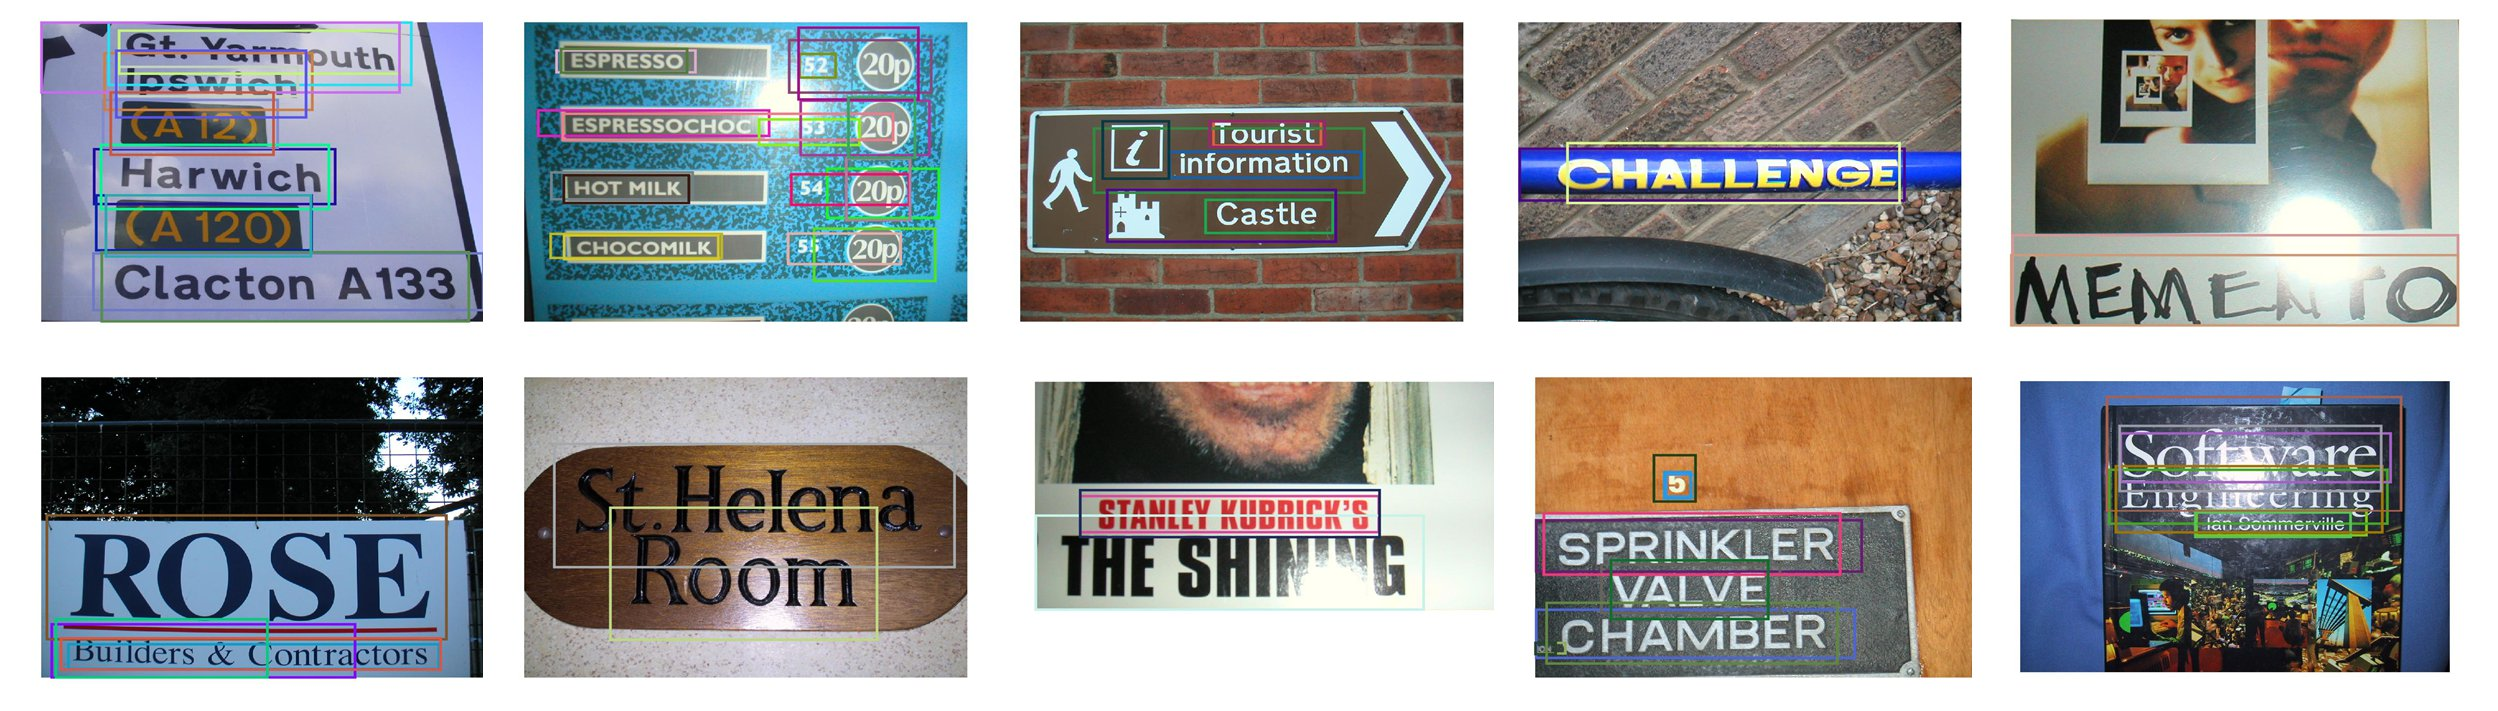
\includegraphics[scale=0.38]{figures/text_lines_proposals}
\caption{ICDAR2011~\cite{shahab2011icdar}上的文本行检测结果,不同颜色的窗口表示不同的文本行。}
\label{fig:text_prop}
\end{figure}

为了定量评价本文所提出的方法在文本行检测上的性能,我们采用了和~\cite{Zhang15}一样的“字符检测率”(character detection rate)作为评价标准:
\begin{equation}
R = \frac{\sum_{i=1}^N\sum_{j=1}^{|G_i|}\text{max}_{k=1}^{|D_i|}M_s(G^{(j)}_i, D^{(k)}_i)}{\sum_{i=1}^N|G_i|}
\end{equation}
上式中$N$是数据集中图像的数目,$G^{(j)}_i$和$D^{(k)}_i$分别表示第$i$张图像的ground-truth和检测出的窗口,$M_s(G^{(j)}_i, D^{(k)}_i)$是第$j$个ground-truth窗口$G^{(j)}_i$和第$k$个检测窗口$D^{(k)}_i$的“匹配度”,通过以下公式计算:
\begin{equation}
M_s(G^{(j)}_i, D^{(k)}_i) = 
\begin{cases}
1 \ \text{if} \ \frac{|G^{(j)}_i \cap D^{(k)}_i|}{|G^{(j)}_i|} \geq 0.8 \ \text{and}\ \frac{\max(h(G^{(j)}_i),h(D^{(k)}_i))}{\min(h(G^{(j)}_i),h(D^{(k)}_i))} \leq 2.5 \\
0 \ \text{otherwise}
\end{cases}
\label{eq:text_ms}
\end{equation}
式~\ref{eq:text_ms}中$w(\cdot)$和$h(\cdot)$分别是文本行区域的宽和高。我们将本文所提出的方法和~\cite{Zhang15}进行对比,~\cite{Zhang15}是一个利用对称性进行文本行检测的方法。图~\ref{fig:character_detection_rate}是对比结果,本文所提出方法比~\cite{Zhang15}得到了更高的字符检测率。
\begin{figure}[H]
\centering
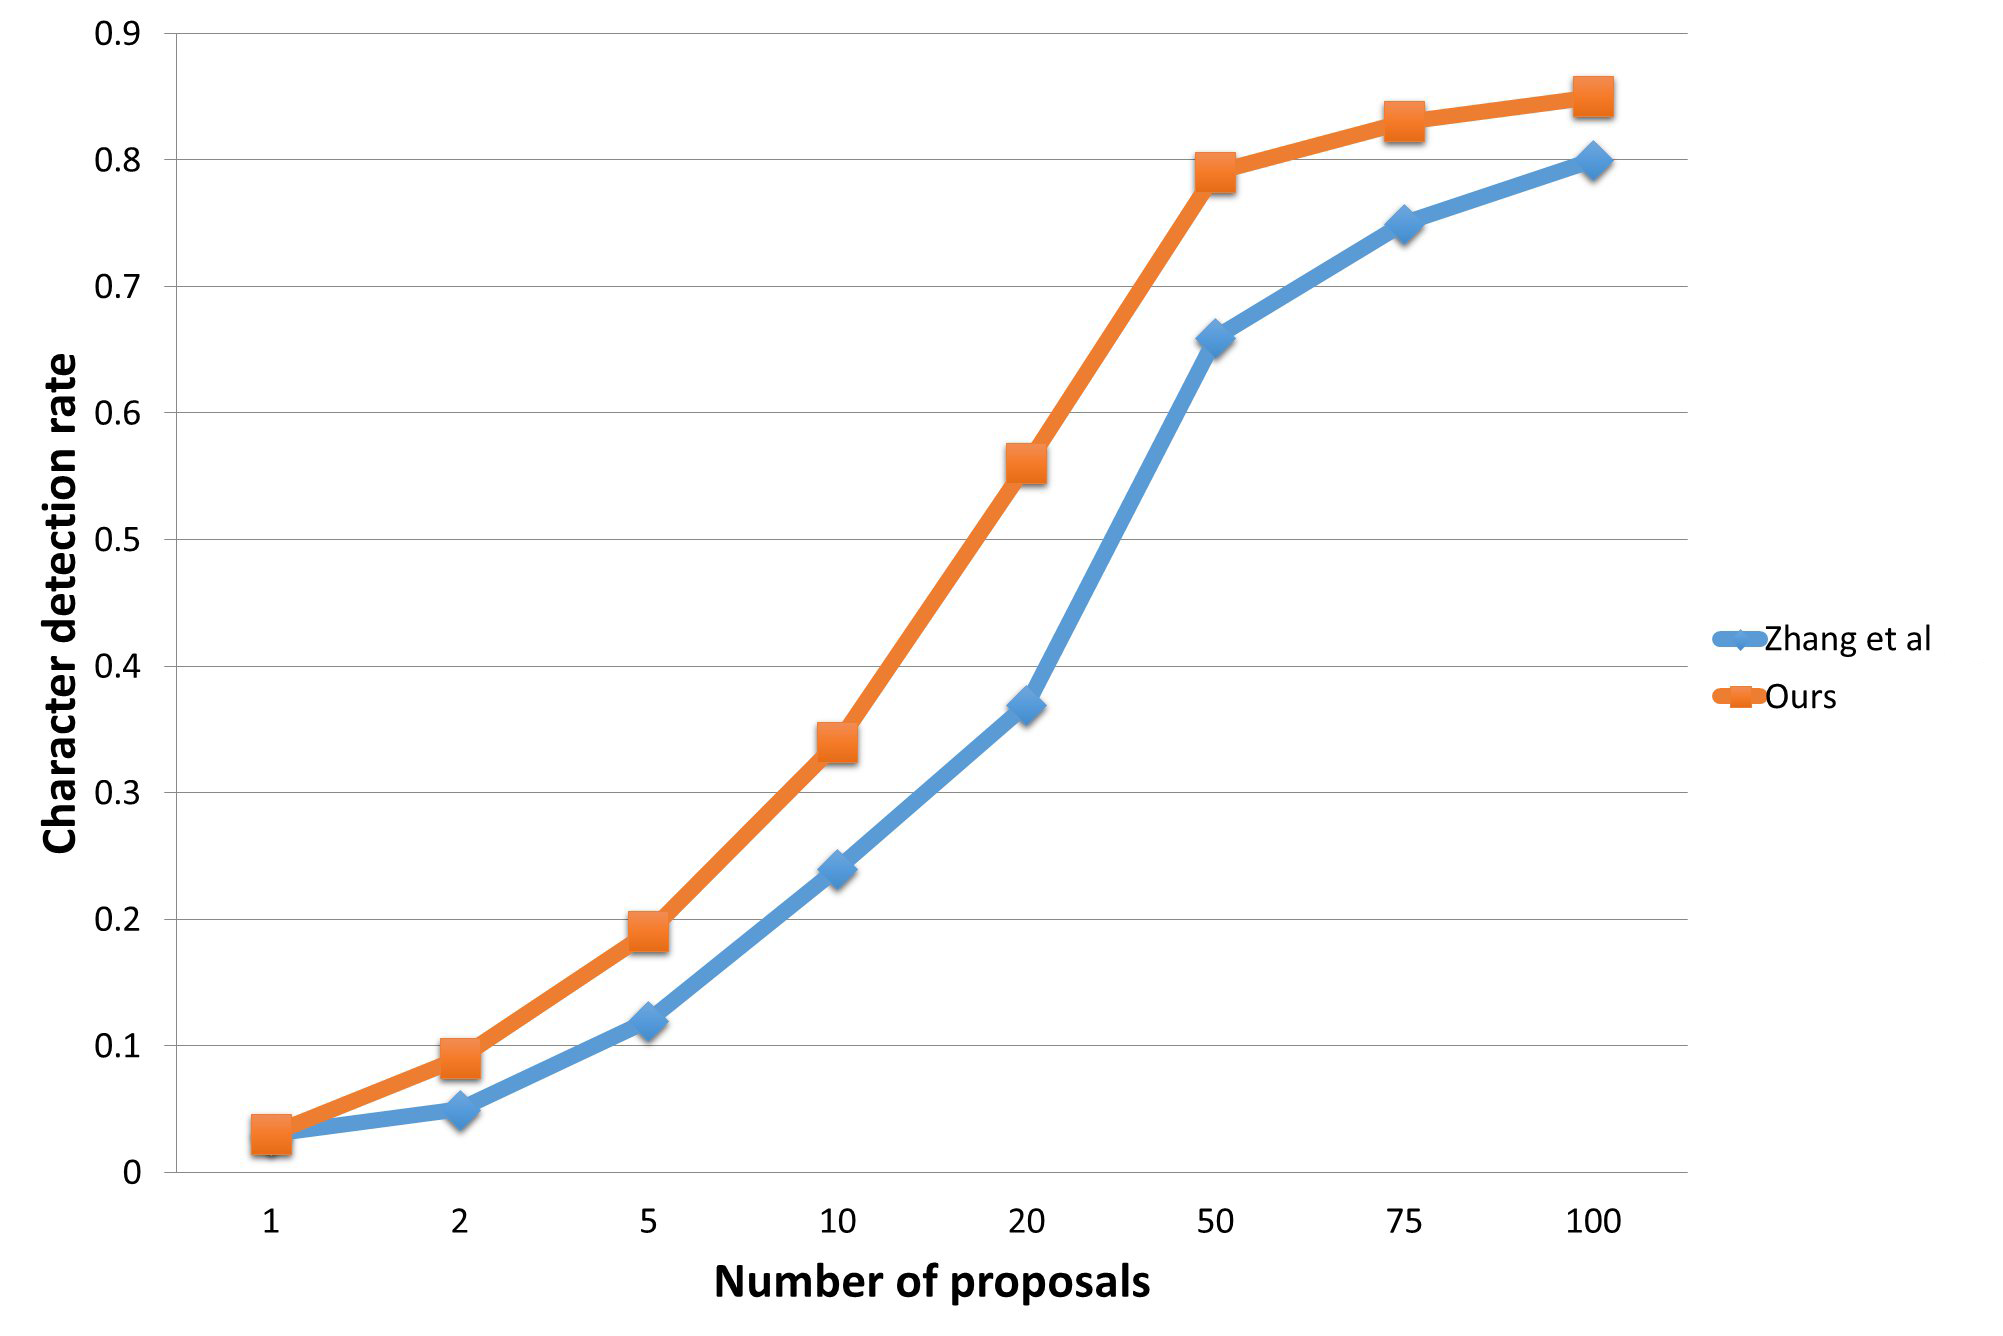
\includegraphics[scale=0.3]{figures/character_detection_rate}
\caption{本文所提出的文本行检测方法和~\cite{Zhang15}的字符检测率。}
\label{fig:character_detection_rate}
\end{figure}




\subsection{本章小结}
本章介绍了骨架提取的四个应用:基于骨架的物体分割、基于骨架的候选窗口检测、航拍图中道路检测和自然图像中文本行检测。在 WH-SYMMAX 和 SK-LARGE 两个公开数据集上的实验结果表明本章所提出算法的分割结果具有明显优势,甚至优于基于深度学习的图像分割算法,
这说明所提出的多任务网络能够在准确检测骨架的同时预测骨架尺度。由于训练时的监督并没有任何类别相关信息,骨架人工标注成本也低于语义分割的逐像素标注,因此本文所提出的分割算法无论在性能还是可拓展性上都具有明显优势。
基于骨架的候选窗口检测算法通过修正 Edge Boxes 算法的候选窗口似物性得分,抑制了位于图像背景和不能完全包含物体的候选窗口,得到了重排序的高质量候选窗口。在ETHZ Shape Classes~\cite{ferrari2006object}数据集上的实验结果表明
增加骨架信息可以明显提升Edge Boxes候选窗口检测算法的性能。

由于航拍图中的道路和自然图像中的文本行具有对称性,因此本文所提出骨架检测算法也适用于道路和文本行检测。在一个航拍图数据集和文字检测的权威数据集ICDAR2011上的对比实验结果表明,本文所提出的方法在对称物体的检测上也有明显优势。

本章所介绍的几个应用说明骨架作为一种物体形状的高级简洁的表示,对物体检测、文本检测等其它计算机视觉任务有促进作用。本章研究内容已发表在计算机视觉领域国际顶级会议“IEEE Conference on Computer Vision and Pattern Recognition 2016”和由爱思唯尔(Elsevier)出版的学术专著“Skeletonization: Theory, Methods, and Applications”中的一章“Skeletonization in Natural Images and Its Application to Object Recognition”。

%%%%%%%%%%%%%%%%%%%%%%%%%%%%%%%%%%%%%%%%%%%%%%%%%%%%%%%%%%%%%%%%%%%%%%%%%%%%%%%%%%%
%%%%%%%%%%%%%%%%%%%%%%%%%%%%%%%%%%%%%%%%%%%%%%%%%%%%%%%%%%%%%%%%%%%%%%%%%%%%%%%%%%%
\pagebreak
\section{总结与展望}
\subsection{全文总结}
骨架是一种高级抽象的物体表示方法,由于其包含了物体的形状特征和部件连接的拓扑结构信息,在基于形状的物体检测与识别中具有独一无二的优势。骨架提取和其相关的研究一直是计算机视觉领域的热点。从自然图像中直接提取骨架是一个极具
挑战性的问题,因为自然图像中1)背景复杂,2)前景物体多变,3)骨架尺度未知。本文以自然图像中的物体骨架检测为核心展开,提出了基于多尺度边输出的多任务网络用于骨架提取,并用所提取出的骨架恢复出物体分割、提取目标检测的候选窗口和检测对称物体,
展现了骨架提取在计算机视觉其他领域的应用潜力。本文的具体工作概括如下:

1)提出了基于尺度相关的边输出(SSO:scale-associated side-output)网络,利用神经网络不同感受野的卷积层的输出(边输出side-output)解决骨架检测中的尺度未知难题,并进一步拓展为多任务网络,同时检测物体骨架和预测骨架尺度,在得到
骨架尺度的同时提升骨架检测的性能;

2)提出了一种利用骨架和骨架尺度进行物体分割的算法,由于骨架包含物体部件连接信息和形状信息,而骨架尺寸补充了物体形状的大小信息,利用作以骨架为中心,骨架尺度为半径的圆可得到物体的分割;

3)提出了基于骨架的候选窗口提取算法,由于目标一般位于图像前景,根据所检测骨架和得到的分割可抑制现有候选窗口提取算法产生的位于背景上的干扰窗口,提高候选窗口提取算法的性能;

4)介绍了用所提出骨架检测算法在对称物体检测上的应用,如航拍图中的道路检测和自然图像中的文本行检测。

本文的主要工作,第一点主要致力于自然图像中骨架提取这一基础工作,同时本文提出的多任务网络能够在提取骨架的同时得到骨架尺度;第二、三、四点主要是骨架的应用,即根据骨架和骨架尺度得到物体分割、利用骨架检测候选窗口以及基于对称性的图像中目标检测。

\subsection{对未来工作的展望}
本文对自然图像中的骨架提取和其应用作了深入的研究,所提出的方法均通过大量实验与当前的主流方法进行比较,验证了所提出方法的优越性,对骨架识别和相关研究有推动作用。但是仍有很多有待深入挖掘的内容可以提升骨架提取的性能:

1).利用骨架在空间上的先验改善检测结果。从图~\ref{fig:examples_skl}的检测结果可以看到,现有的大部分方法的检测结果仍然普遍存在骨架不连续和不平滑的情况,利用骨架本身在空间上的先验信息可以对检测到的骨架进行后处理,使得检测结果
更加连续和平滑。

2).学习“非极大值抑制”进行骨架细化,完成真正的端到端检测。正如1)中所述,现有方法检测到的骨架普遍存在不连续不平滑的现象,这一部分原因是使用“非极大值抑制”对检测到的骨架进行细化时造成的,模型输出的原始概率图实际上是相对比较
平滑的(图~\ref{fig:fsds_hed})。将“非极大值抑制”嵌入到学习模型中,让模型自动学习这一过程,可能会得到更好的骨架细化结果。

%% 参考文献
\pagebreak
\bibliographystyle{ieeetr}
\addcontentsline{toc}{section}{参考文献}
\bibliography{master-thesis}

%%%%%%%%%%%%%%%%%%%%%%%%%%%%%%%%%%%%%%%%%%%%%%%%%%%%%%%%%%%%%%%%%%%%%%%%%%%%%%%%%%%
%%%%%%%%%%%%%%%%%%%%%%%%%%%%%%%%%%%%%%%%%%%%%%%%%%%%%%%%%%%%%%%%%%%%%%%%%%%%%%%%%%%
\pagebreak
\section*{作者在攻读硕士学位期间公开发表的论文}
\addcontentsline{toc}{section}{作者在攻读硕士学位期间公开发表的论文}
%\nobibliography*
\begin{enumerate}
\item “Object Skeleton Extraction in Natural Images by Fusing Scale-associated Deep Side Outputs",in \emph{Proceedings of the IEEE Conference on Computer Vision and Pattern Recognition}, June 2016.
(IEEE CVPR为模式识别和计算机视觉的三大国际顶级会议,中国计算机协会列为A类会议,根据2017年谷歌学术统计,h5-index排名所有学术刊物第35位,位列工程和计算机领域所有学术刊物第一位。)

\item “Skeletonization in Natural Images and Its Application to Object Recognition" in "\textbf{ Skeletonization: Theory, Methods, and Applications }", Punam Saha, Gunilla Borgefors, Gabriella Sanniti di Baja (Ed.), 
Academic Press, 2017. ISBN: 978-0-081-01291-8. (本书为爱思唯尔 Elsevier出版的学术专著。)

\item “DeepSkeleton: Learning Multi-task Scale-associated Deep Side Outputs for Object Skeleton Extraction in Natural Images",in \emph{IEEE Transactions on Image Processing}, 2017.(注:第二作者,导师第一作者。IEEE TIP是中国计算机协会A类、图像处理领域的顶级期刊,SCI II区。)

\item “Label Distribution Learning Forests",in \emph{Proceedings of Advances in neural information processing systems}, 2017.(注:NIPS 是机器学习领域的顶级会议、中国计算机协会A类会议。)

\item “基于对称轴的自然图像中物体部件检测”,《中国科技论文》第14期。

\end{enumerate}
%\emph{IEEE Conference on Computer Vision and Pattern Recognition}(\textbf{CVPR}),是计算机视觉领域三大国际顶级会议(CVPR, ECCV, ICCV)之一。

%%%%%%%%%%%%%%%%%%%%%%%%%%%%%%%%%%%%%%%%%%%%%%%%%%%%%%%%%%%%%%%%%%%%%%%%%%%%%%%%%%%
%%%%%%%%%%%%%%%%%%%%%%%%%%%%%%%%%%%%%%%%%%%%%%%%%%%%%%%%%%%%%%%%%%%%%%%%%%%%%%%%%%%
\pagebreak
\section*{作者在攻读硕士学位期间所参与的项目}
\addcontentsline{toc}{section}{作者在攻读硕士学位期间所参与的项目}
\begin{enumerate}
\item 国家自然科学基金(No.61303095),基于有监督学习的自然图像中骨架提取和物体识别研究(2014.1-2016.12)。
\item 上海市教育委员会科研创新项目(No.14YZ018),基于对称性的自然图像中物体表示与识别研究(2014.1-2015.12)。
\item 高等学校博士学科点专项基金(No.20133108120017),基于对称性表示的自然图像中目标定位研究(2014.1-2016.12)。

\end{enumerate}

%%%%%%%%%%%%%%%%%%%%%%%%%%%%%%%%%%%%%%%%%%%%%%%%%%%%%%%%%%%%%%%%%%%%%%%%%%%%%%%%%%%
%%%%%%%%%%%%%%%%%%%%%%%%%%%%%%%%%%%%%%%%%%%%%%%%%%%%%%%%%%%%%%%%%%%%%%%%%%%%%%%%%%%
\pagebreak
\section*{致谢}
\addcontentsline{toc}{section}{致谢}
我要真诚地感谢硕士阶段的导师沈为老师,在本文撰写和平时科研上他都给了我详尽和具体的指导。沈老师一开始就给我们设定了很高的要求,以发表顶级会议论文为目标,这对我影响深远。

我也要感谢实验室的另外两位老师对我们学习和生活上的关心和支持。张之江老师给了我多次锻炼的机会,去研究生课堂上介绍自己的科研工作,曾丹老师给了我很多关心和鼓励。感谢我的师弟师妹,还有实验室的其他同学帮我跑实验、准备数据。

最后感谢我的父母对我的支持和付出。
\end{document}
